\clearpage
\subsection{Seismic}
\begin{table}[h!]
\centering
\caption{Categorised seismic profile keywords based on geometry, continuity and frequency.}
\begin{tabular}{|p{4.5cm}|p{4.5cm}|p{4.5cm}|}
\hline
\textbf{Geometry / Structure} & \textbf{Continuity} & \textbf{Frequency / Amplitude} \\
\hline
Bowl & Continuous & High amplitude \\
Chaotic & Discontinuous & High frequency \\
Clinoforms & High continuity & Low amplitude \\
Concave & Low continuity & Low frequency \\
Convex & Medium continuity & Medium amplitude \\
Dipping & Moderate continuity & Medium frequency \\
Downlap & Poor continuity & Moderate amplitude \\
Draping & Semi-continuous & Varied frequency \\
Faulting & Semi-chaotic & \\
Horizontal & & \\
Hyperbolic & & \\
Inclined & & \\
Incision & & \\
Lateral & & \\
Onlap & & \\
Lenticular & & \\
Linear & & \\
Mounded & & \\
Oblique & & \\
Planar & & \\
Prograding & & \\
Parallel & & \\
Semi-parallel & & \\
Shingled & & \\
Sheeted & & \\
Sigmoidal & & \\
Sloping & & \\
Progradation/aggradation & & \\
Tabular & & \\
Tangential & & \\
Toplap & & \\
Truncation & & \\
U-shaped & & \\
Undulate & & \\
Wavy & & \\
Subparallel & & \\
\hline
\end{tabular}
\label{tab:separated_keywords}
\end{table}

\subsubsection{Marine}
\begin{figure}[ht!]
    \centering
    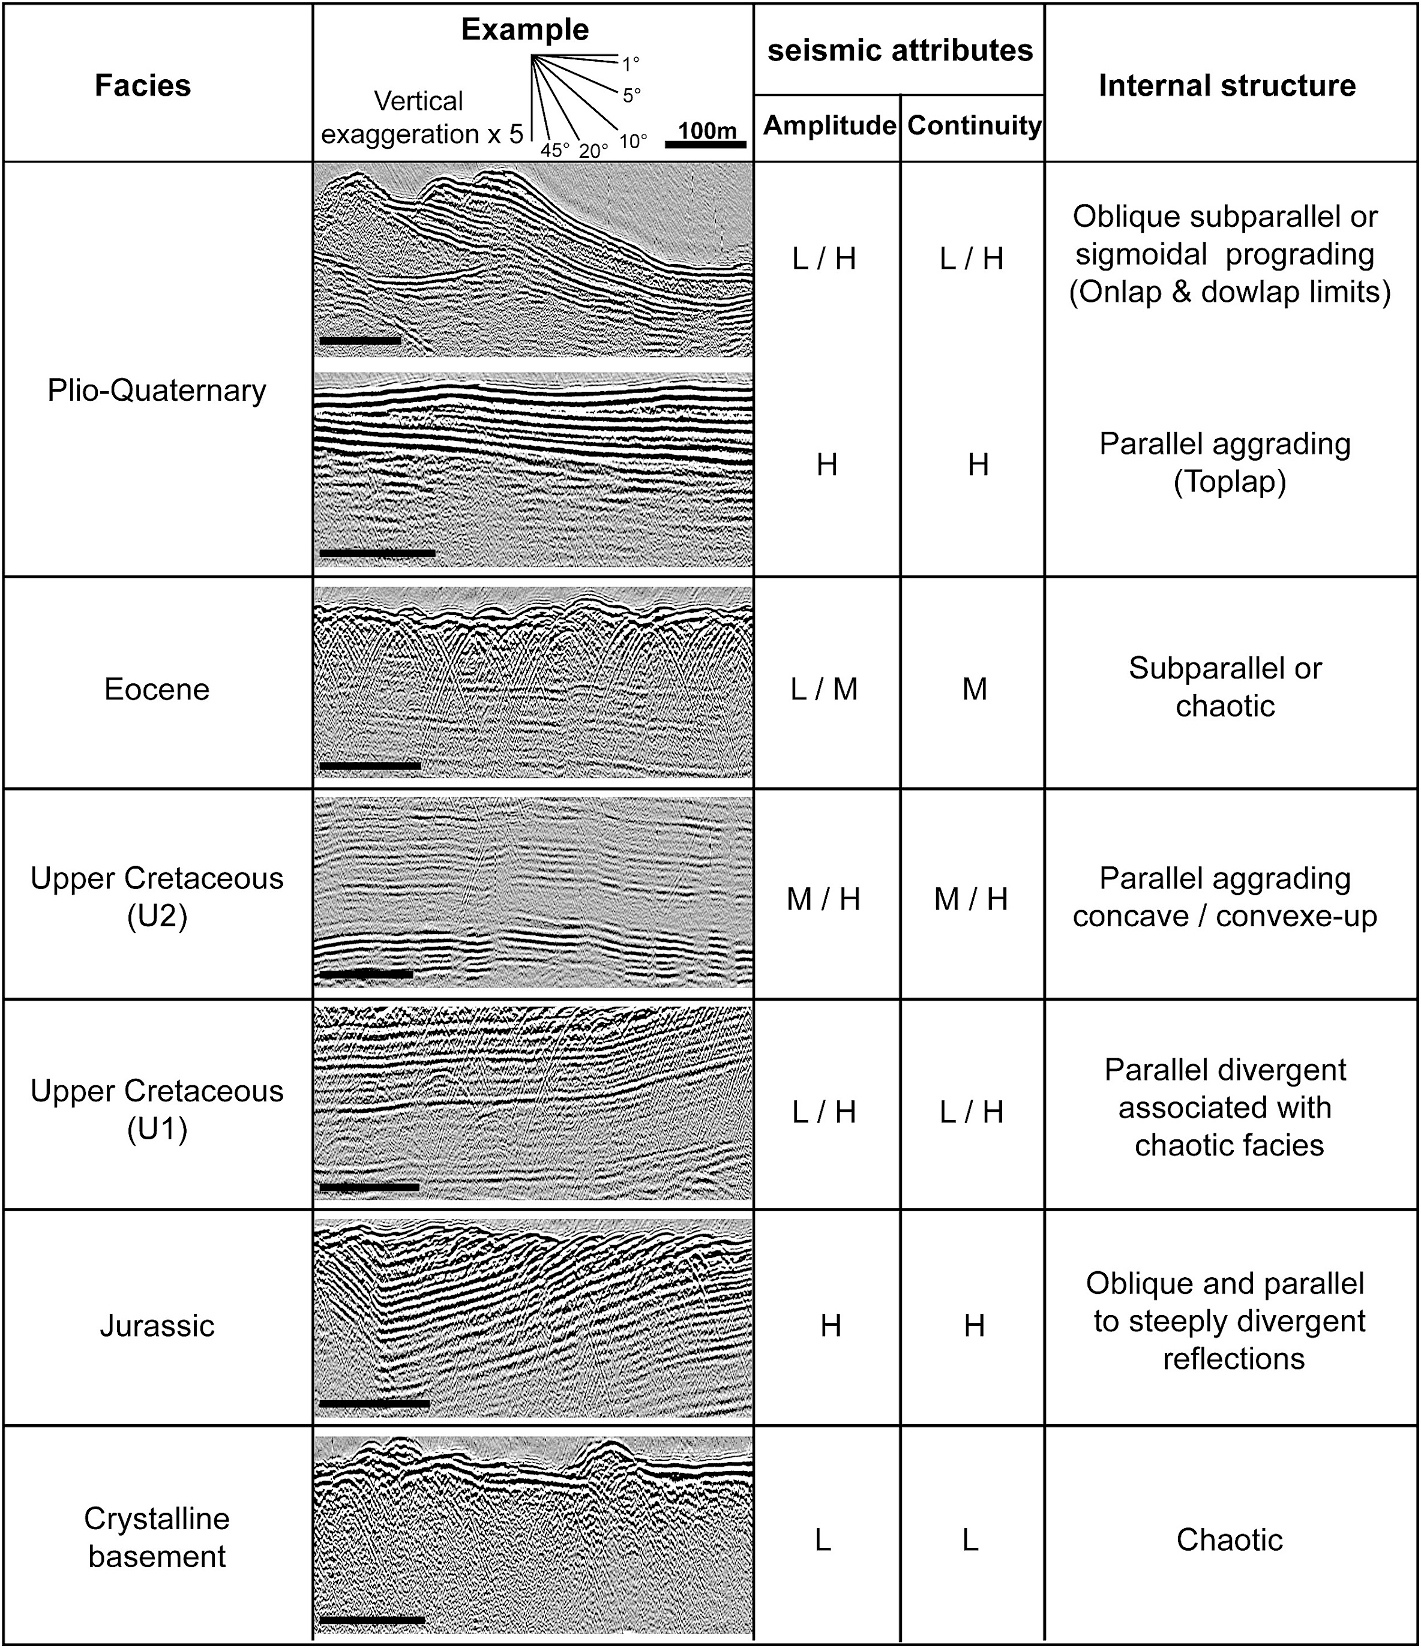
\includegraphics[width=0.9\linewidth]{Figures/0.2GPR/Kaci2024_shelf.png}
    \caption[Structural history of inner shelf.]{Structural history of inner shelf. \textbf{Keywords:}Low continuity, high continuity, oblique, subparallel, sigmoidal, prograding, onlap, downlap, parallel aggrading, toplap, chaotic, concave, convex, divergent, dipping \citep{Kaci2024}.}
    \label{fig:Kaci2024-1}
\end{figure}

\begin{figure}[h!]
    \centering
    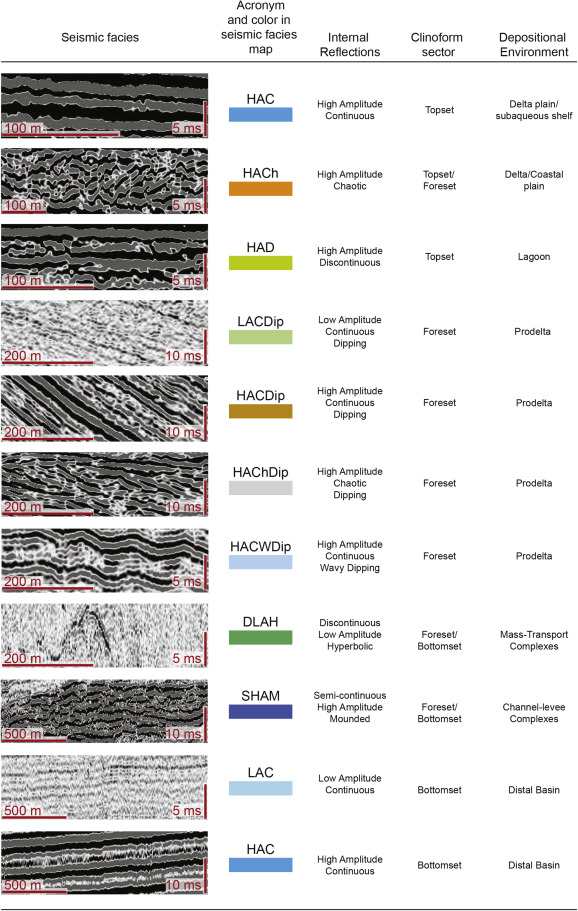
\includegraphics[width=0.9\linewidth]{Figures/0.3Seismic/Pellegrini2018-1.jpg}
    \caption[River lowstand wedge.]{River lowstand wedge. \textbf{Keywords: }High amplitude, low amplitude, continuous, chaotic, discontinuous, dipping, wavy, hyperbolic, semi-continuous, mounded \citep{Pellegrini2018}.}
    \label{fig:Pellegrini2018-1}
\end{figure}

\begin{figure}[h!]
    \centering
    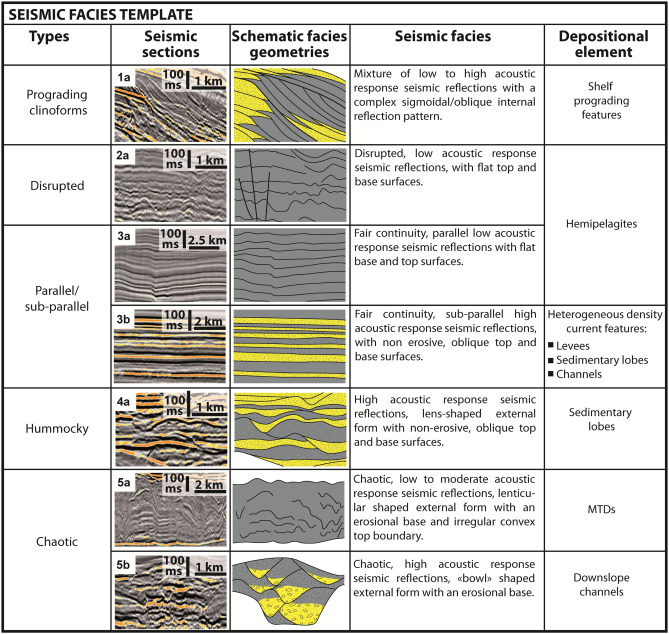
\includegraphics[width=0.9\linewidth]{Figures/0.3Seismic/Thieblemont2020-1.jpg}
    \caption[Channel systems (1).]{Channel systems (1). \textbf{Keywords: }Sigmoidal, oblique, low amplitude, high amplitude, discontinuous, horizontal, continuous, parallel, subparallel, moderate amplitude, lenticular, chaotic, convex, bowl \citep{Thieblemont2020}.}
    \label{fig:Thieblemont2020-1}
\end{figure}

\begin{figure}[h!]
    \centering
    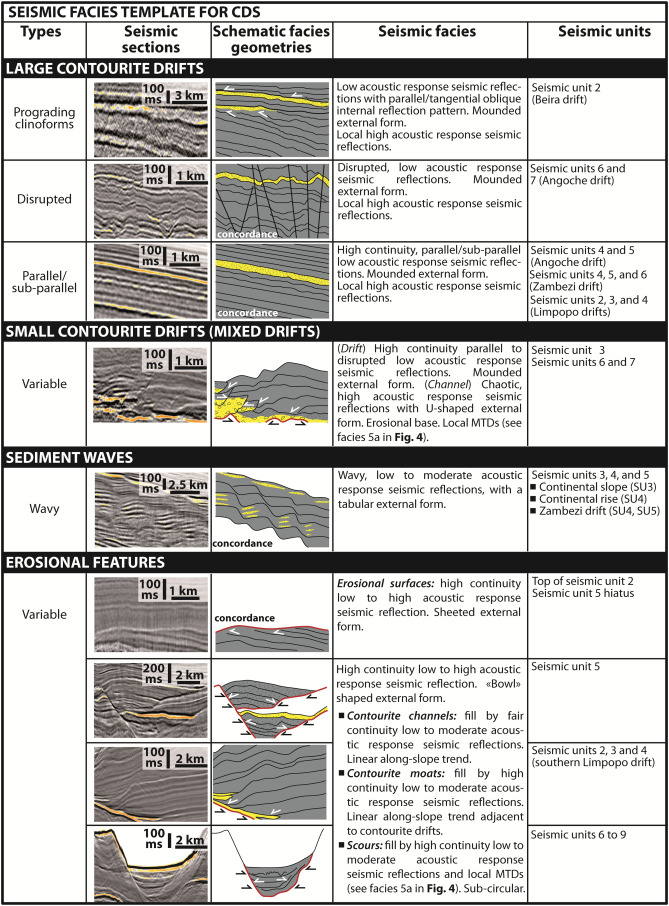
\includegraphics[width=0.9\linewidth]{Figures/0.3Seismic/Thieblemont2020-2.jpg}
    \caption[Channel systems (2)]{Channel systems (2). \textbf{Keywords: }Low amplitude, parallel, tangential, oblique, mounded, high amplitude, discontinuous, continuous, subparallel, chaotic, u-shaped, sheeted, dipping, wavy, moderate amplitude, tabular, bowl, linear \citep{Thieblemont2020}.}
    \label{fig:Thieblemont2020-2}
\end{figure}
\clearpage

\begin{figure}[h!]
    \centering
    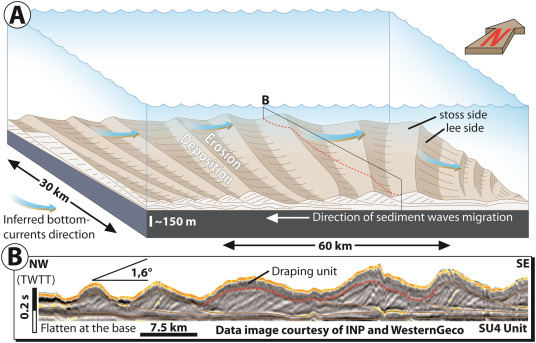
\includegraphics[width=0.75\linewidth]{Figures/0.3Seismic/Thieblemont2020-3.jpg}
    \caption[Channel systems (3).]{Channel systems (3). \textbf{Keywords: } Wavy, dipping, draping, parallel \citep{Thieblemont2020}.}
    \label{fig:Thieblemont2020-3}
\end{figure}

\begin{figure}[h!]
    \centering
    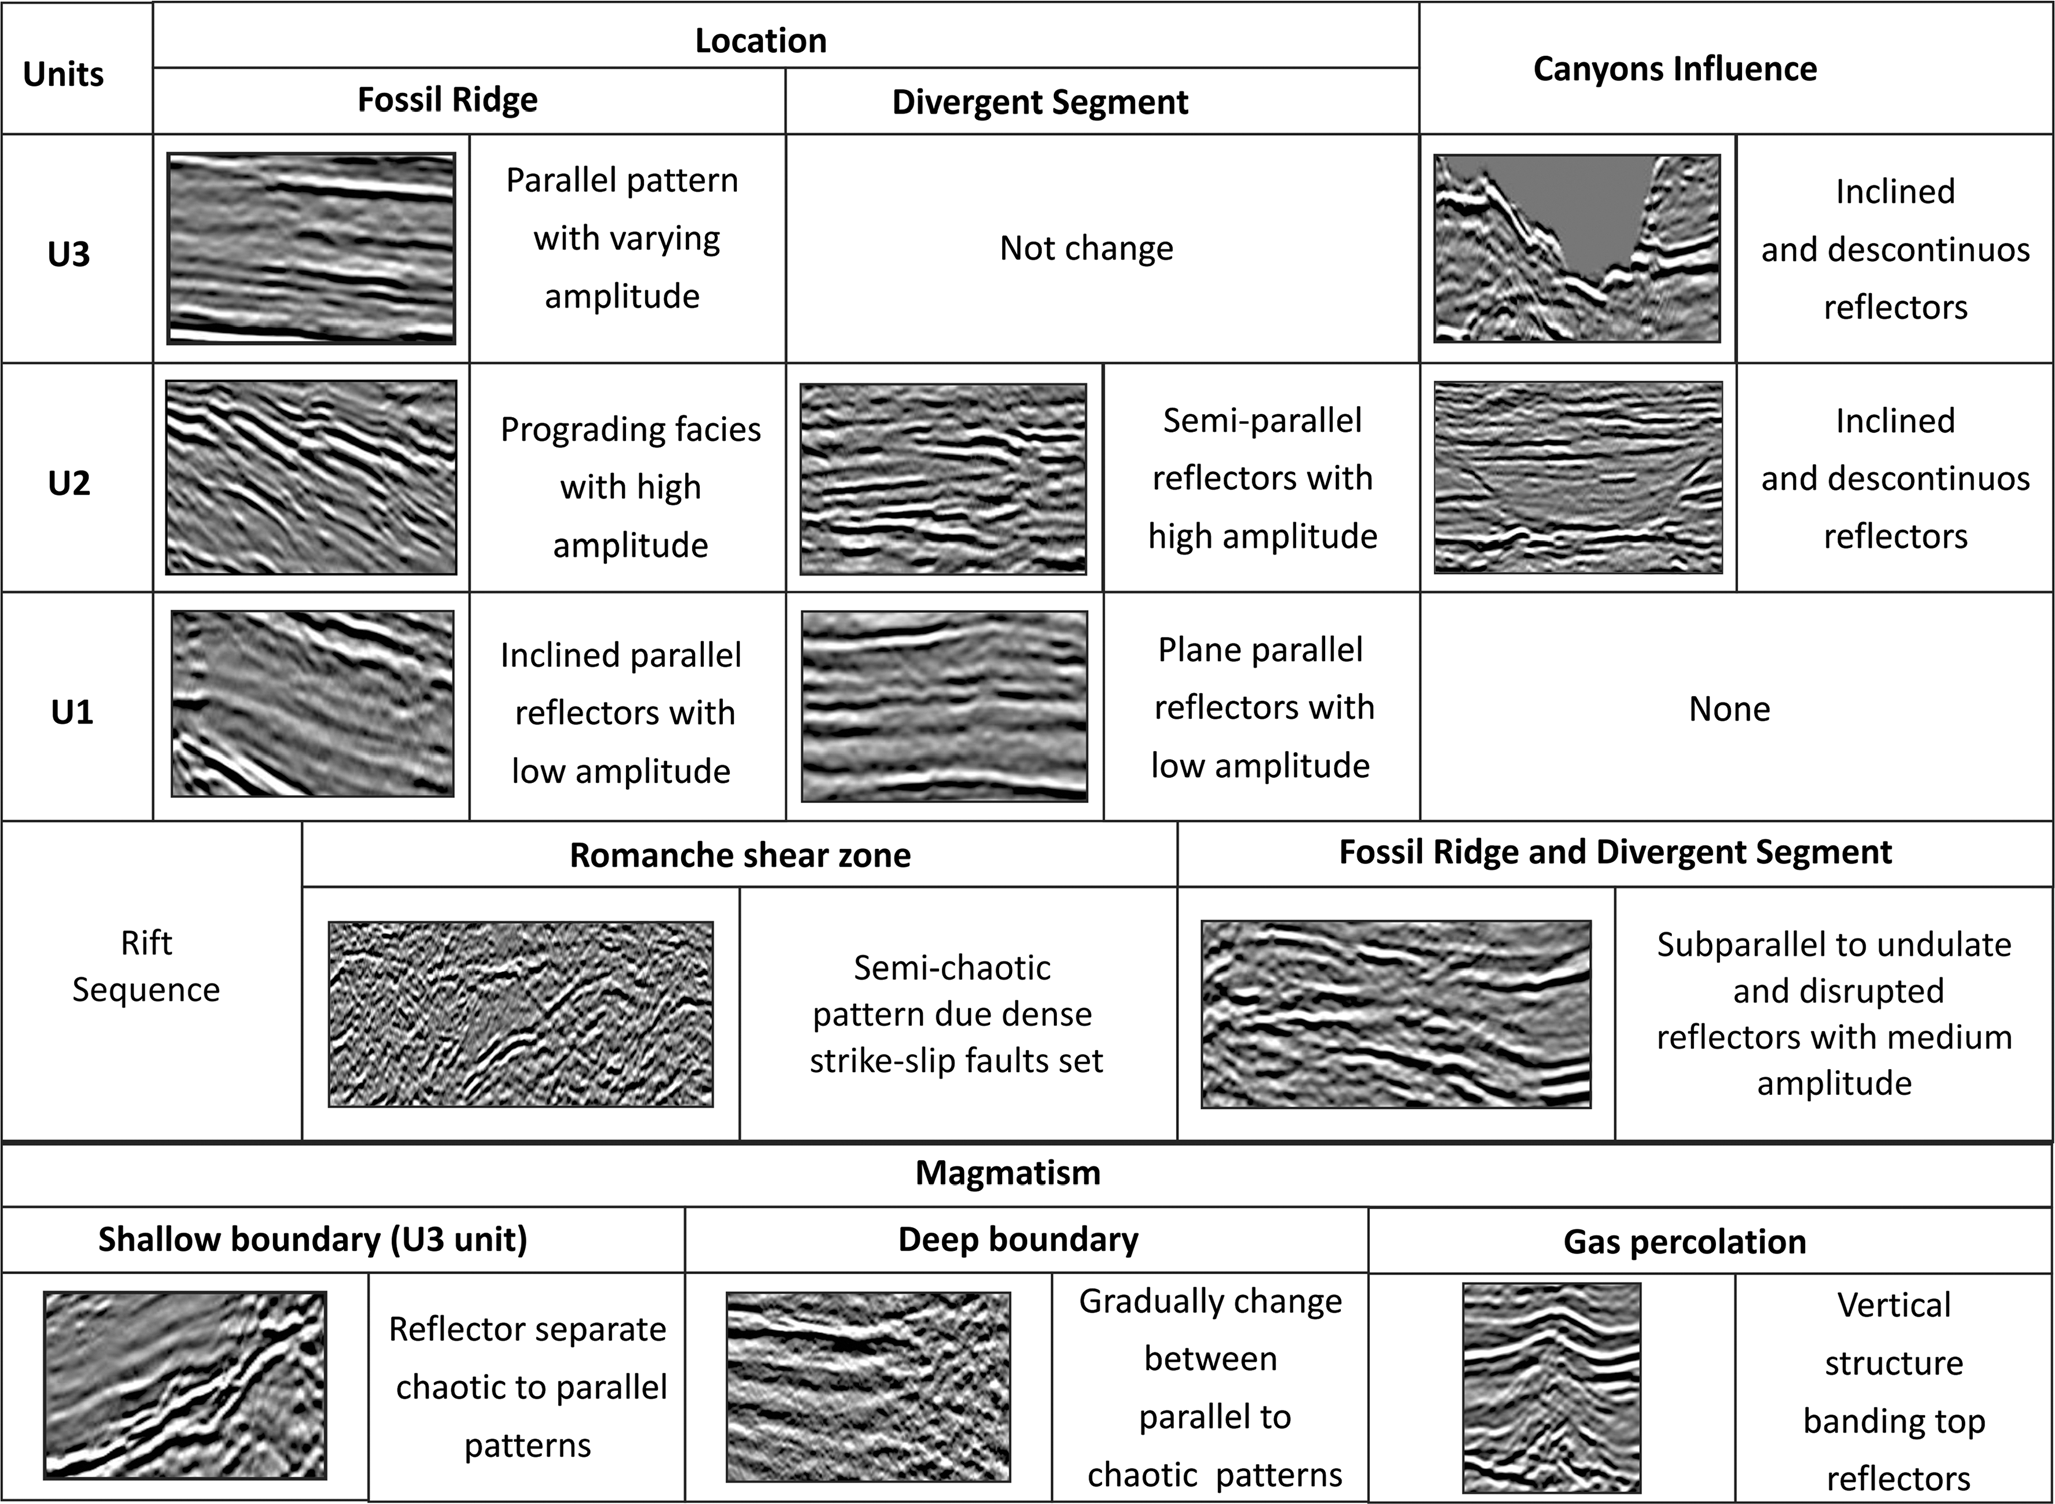
\includegraphics[width=0.75\linewidth]{Figures/0.3Seismic/Andrade2018_trace_1.png}
    \caption[Marginal ridge development.]{Marginal ridge development. \textbf{Keywords: } Parallel, wavy, high amplitude, low amplitude, medium amplitude, planar, semi-parallel, prograding, dipping, inclined, discontinuous, subparallel, chaotic, undulate, faulting, semi-chaotic \citep{Andrade2018}.}
    \label{fig:Andrade2018-1}
\end{figure}

\begin{figure}[h!]
    \centering
    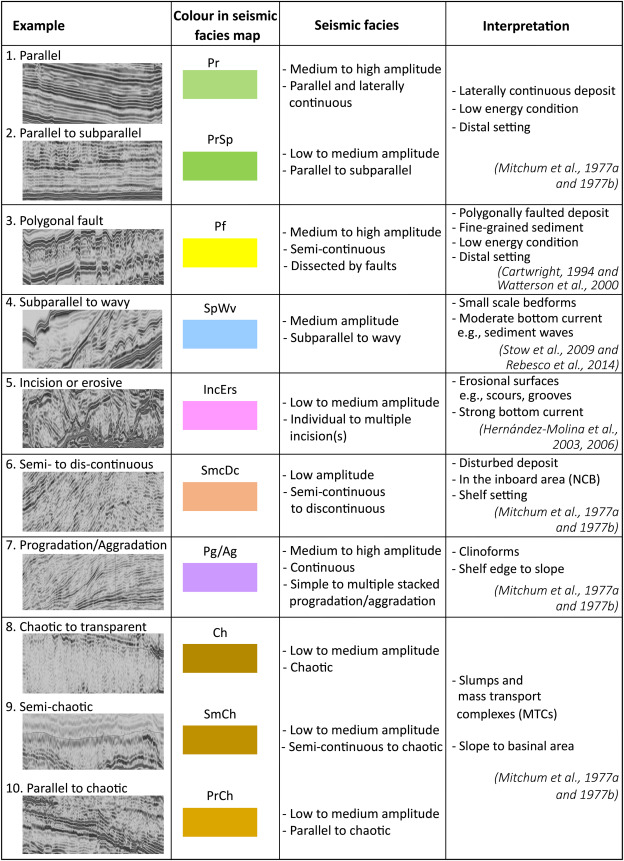
\includegraphics[width=0.9\linewidth]{Figures/0.3Seismic/Winata2023-1.jpg}
    \caption[Passive margin sequences.]{Passive margin sequences. \textbf{Keywords: } Medium amplitude, high amplitude, parallel, lateral, continuous, low amplitude, subparallel, semi-continuous, faulting, wavy, discontinuous, chaotic, incision, stacked progradation/aggradation \citep{winata2023}.}
    \label{fig:Winata2023-1}
\end{figure}

\begin{figure}[h!]
    \centering
    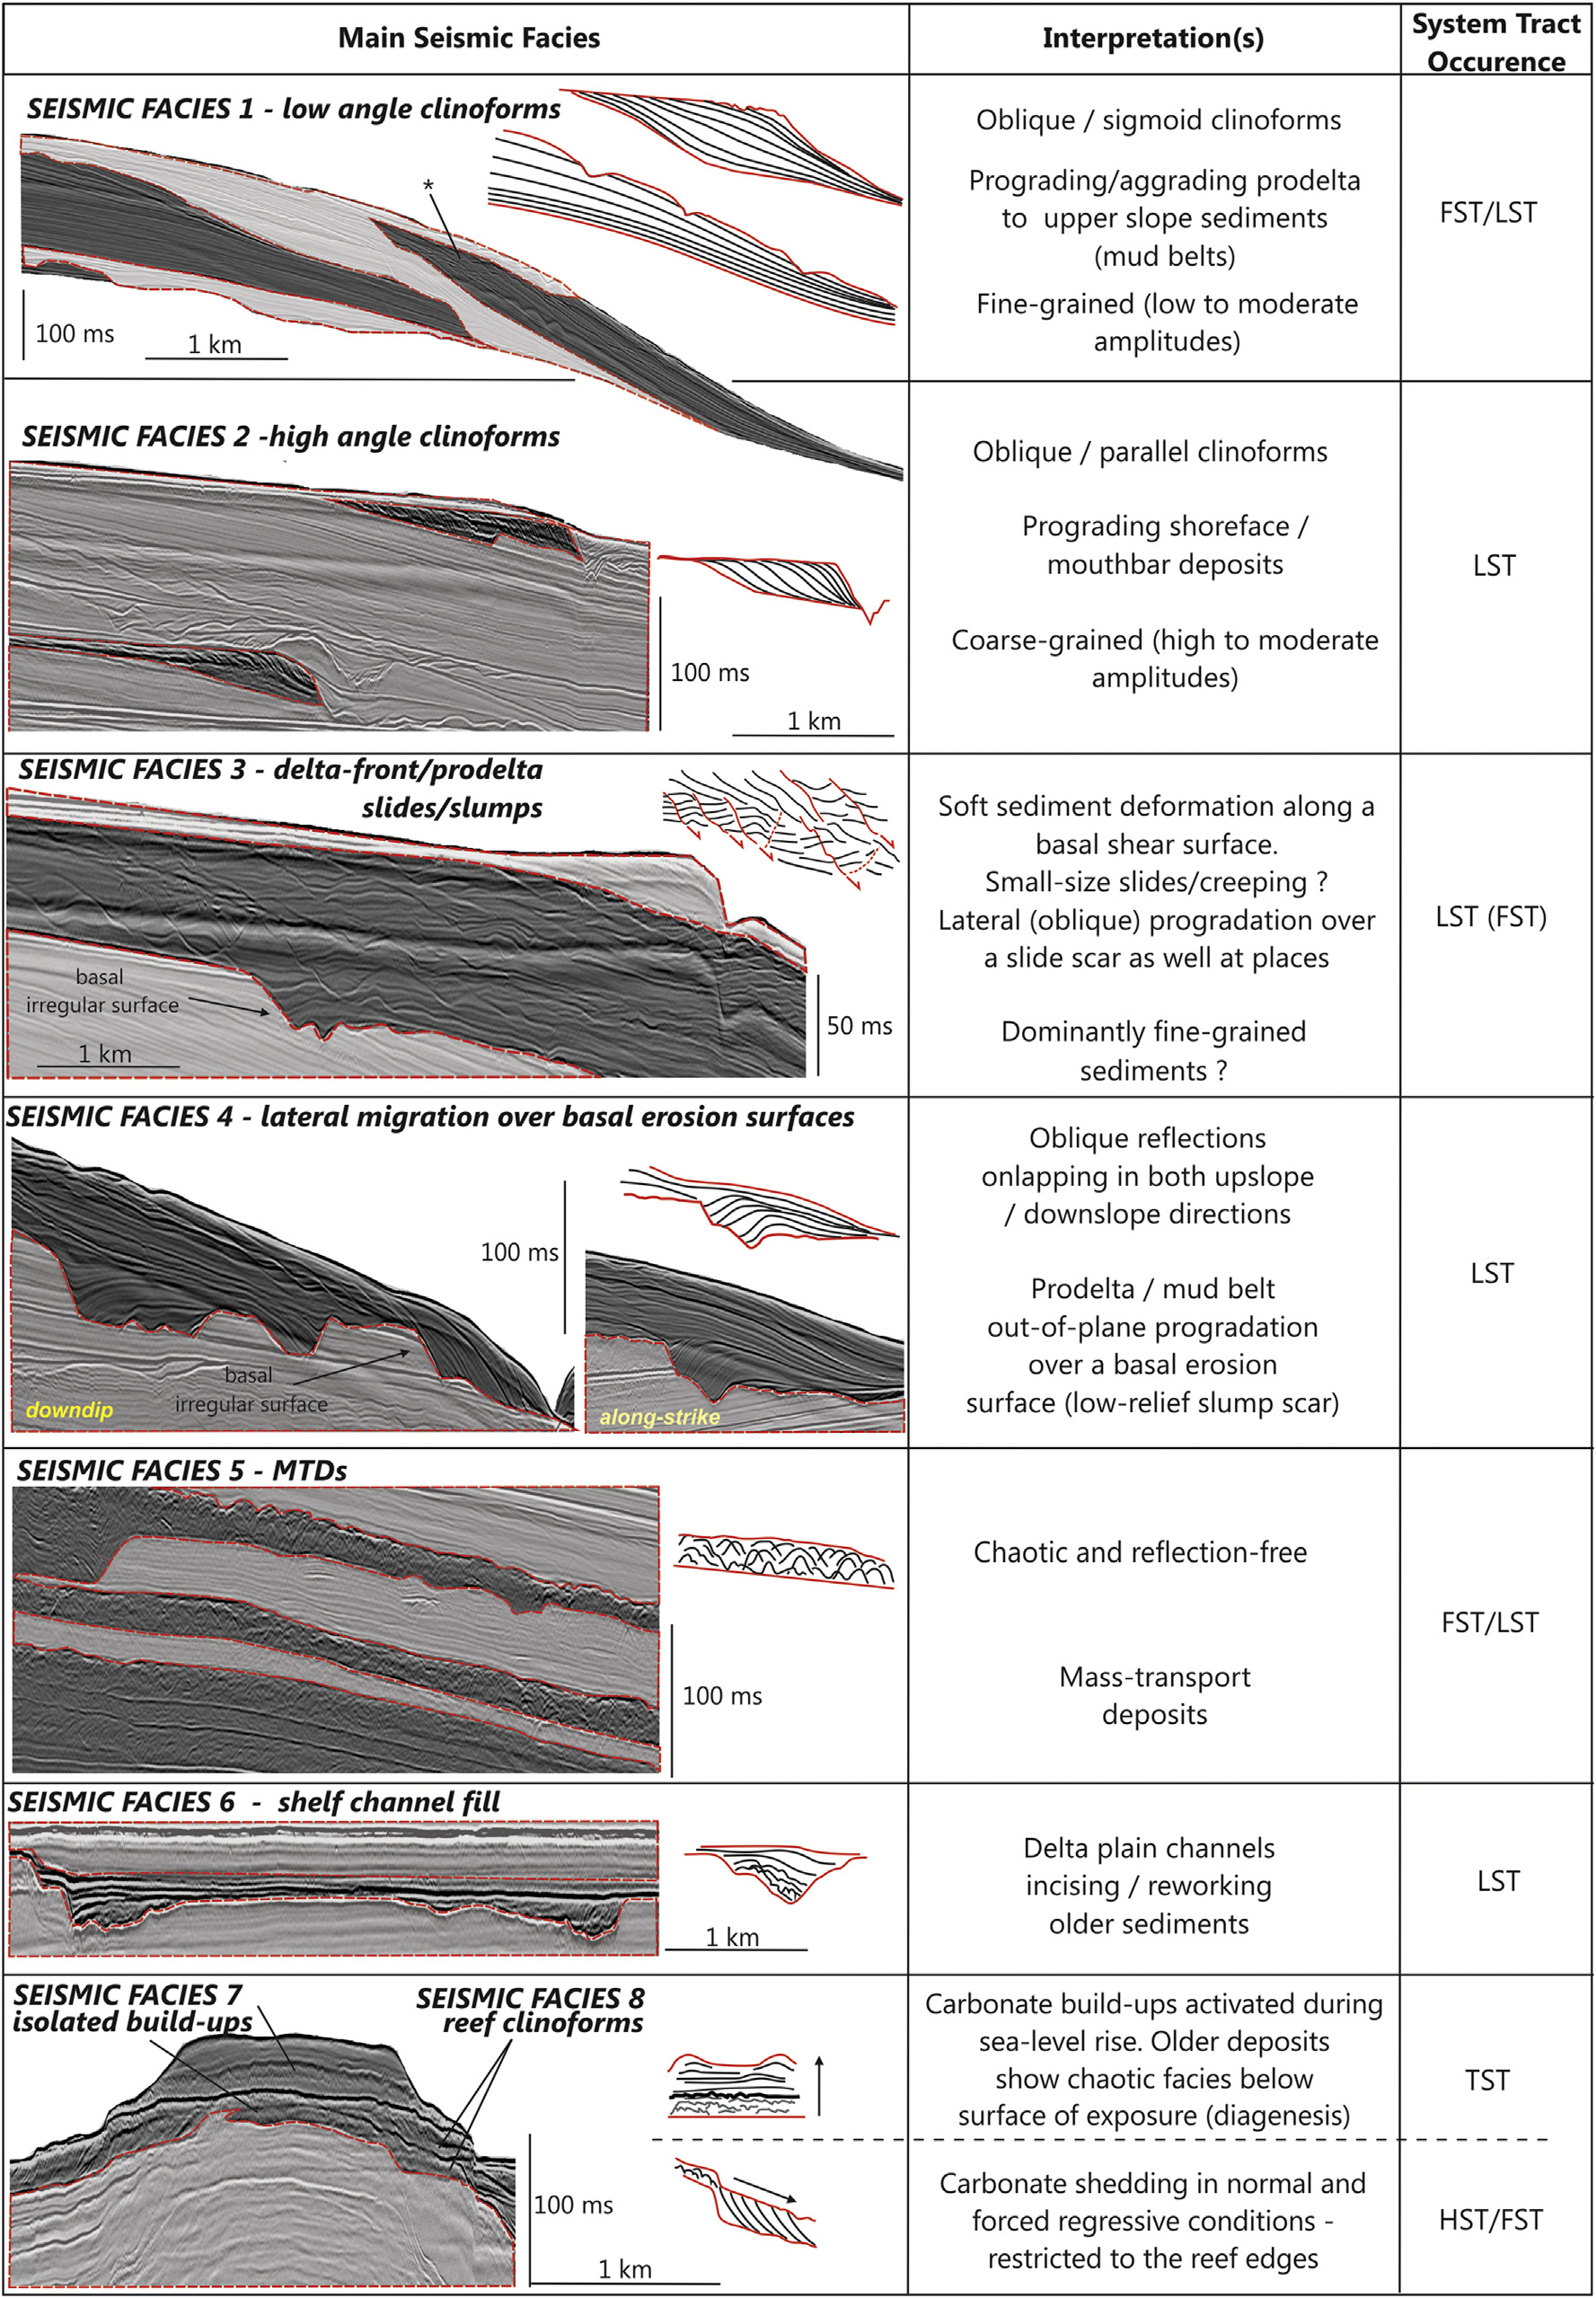
\includegraphics[width=0.9\linewidth]{Figures/0.3Seismic/Bourget2014_trace_1.png}
    \caption[Tide and wave dominated shelf-edge delta.]{Tide and wave dominated shelf-edge delta. \textbf{Keywords: } Oblique, sigmoidal, prograding/aggrading prodelta, sloping, dipping, low amplitude, medium amplitude, parallel, clinoforms, prograding, lateral progredation, onlap, chaotic, horizontal \citep{Bourget2014}.}
    \label{fig:Bourget2014-1}
\end{figure}

\begin{figure}[h!]
    \centering
    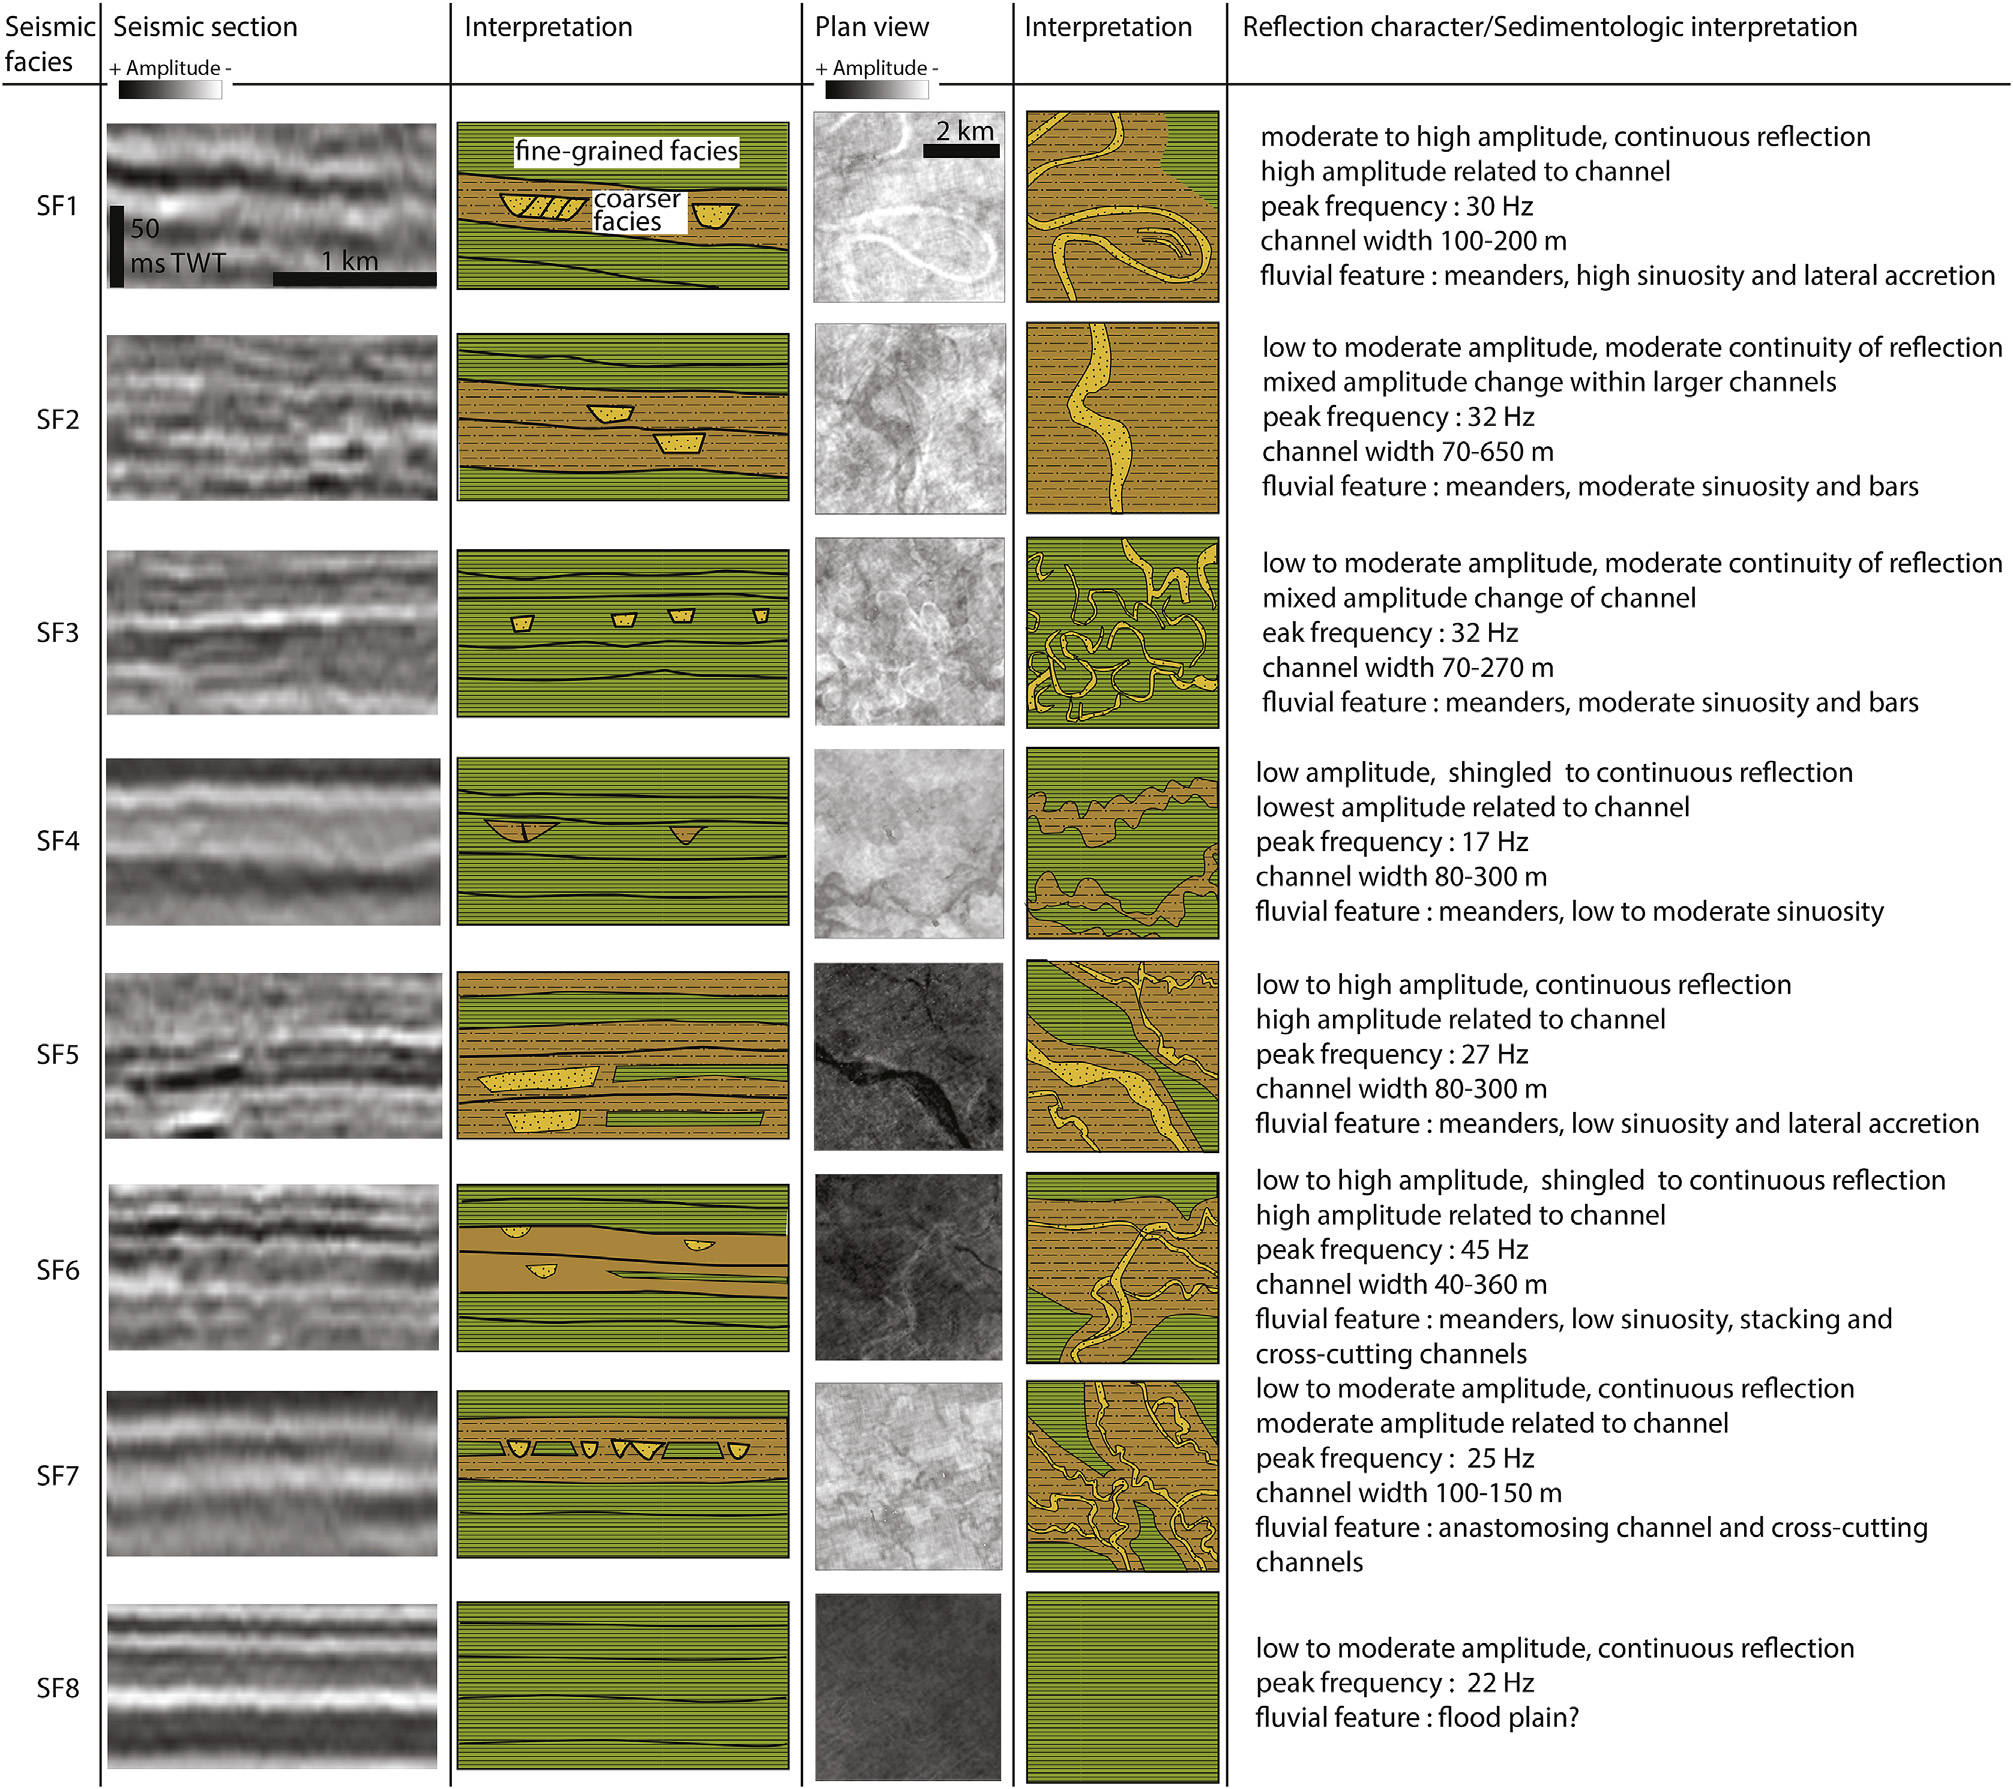
\includegraphics[width=0.9\linewidth]{Figures/0.3Seismic/Calves2019_trace_1.png}
    \caption[Basin fluvial system.]{Basin fluvial system. \textbf{Keywords: } High amplitude, moderate amplitude, continuous, low amplitude, moderate continuity, shingled \citep{Calves2019}.}
    \label{fig:Calves2019-1}
\end{figure}

\begin{figure}[h!]
    \centering
    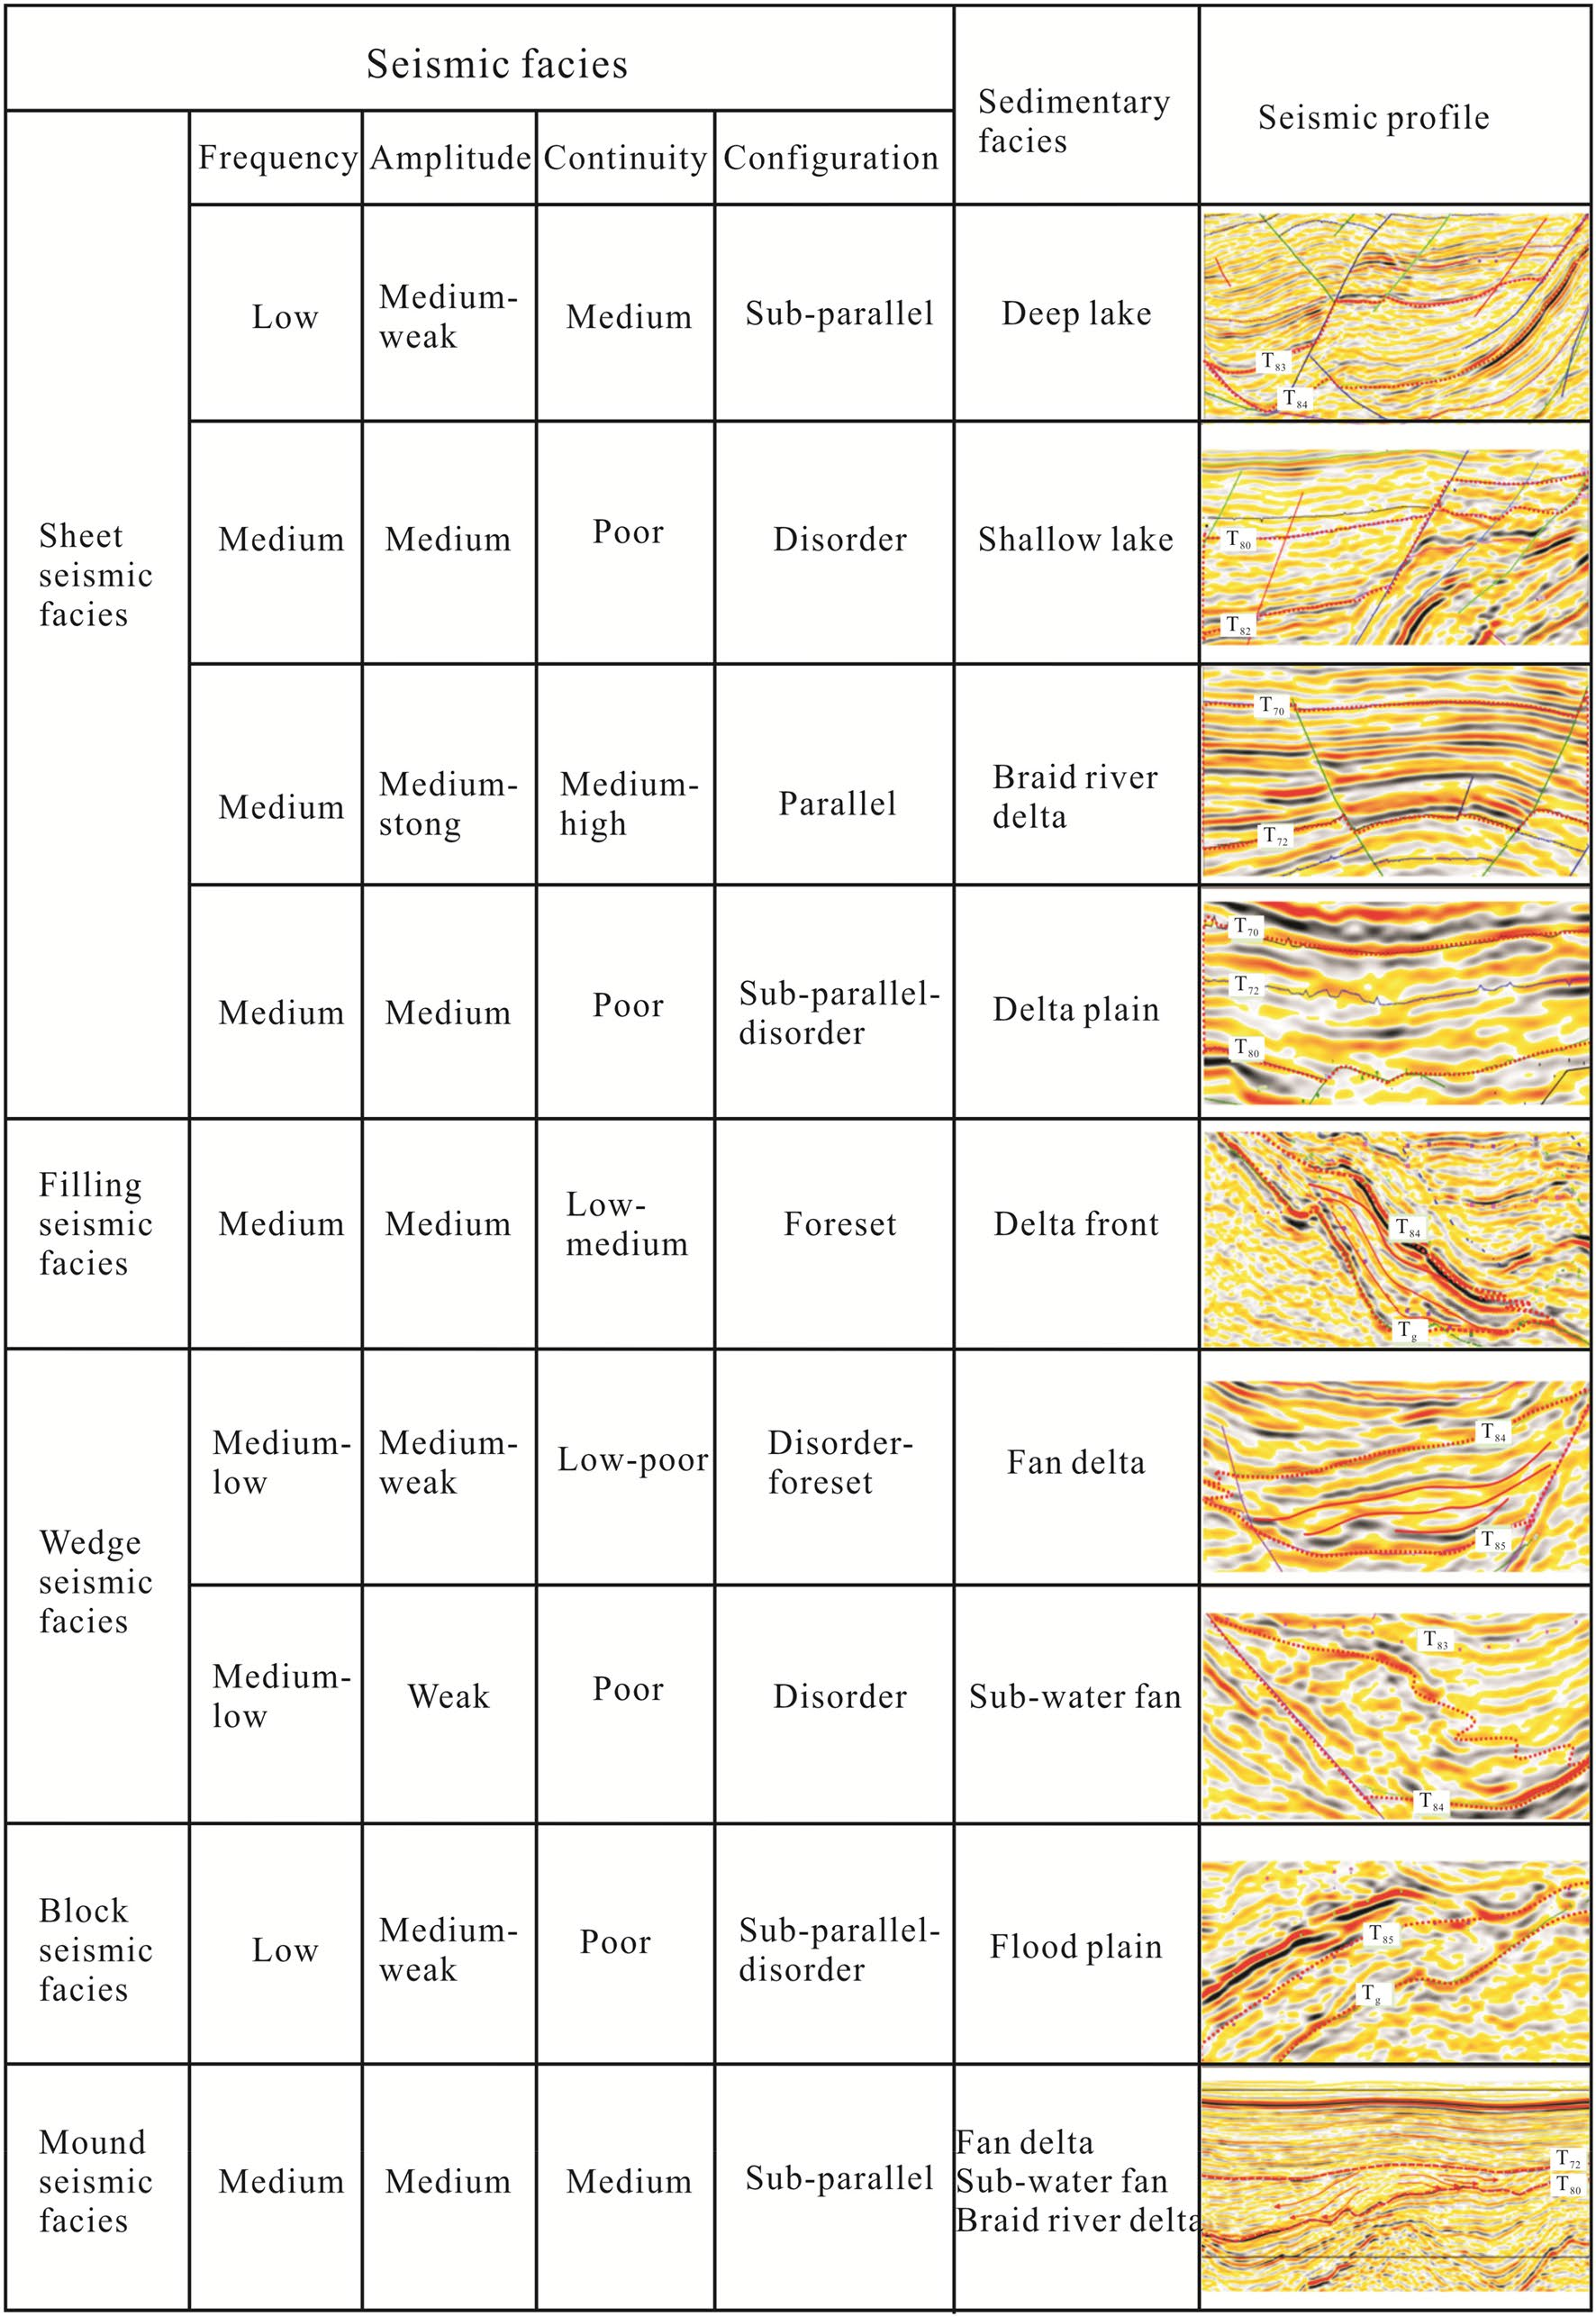
\includegraphics[width=0.9\linewidth]{Figures/0.3Seismic/Chen2017_River_trace_1.png}
    \caption[Eocene sedimentation.]{Eocene sedimentation. \textbf{Keywords: } Low frequency, medium frequency, low amplitude, medium amplitude, high amplitude, poor continuity, medium continuity, low continuity, subparallel, chaotic, parallel, dipping, horizontal \citep{Chen2017}.}
    \label{fig:Chen2017-1}
\end{figure}

\begin{figure}[h!]
    \centering
    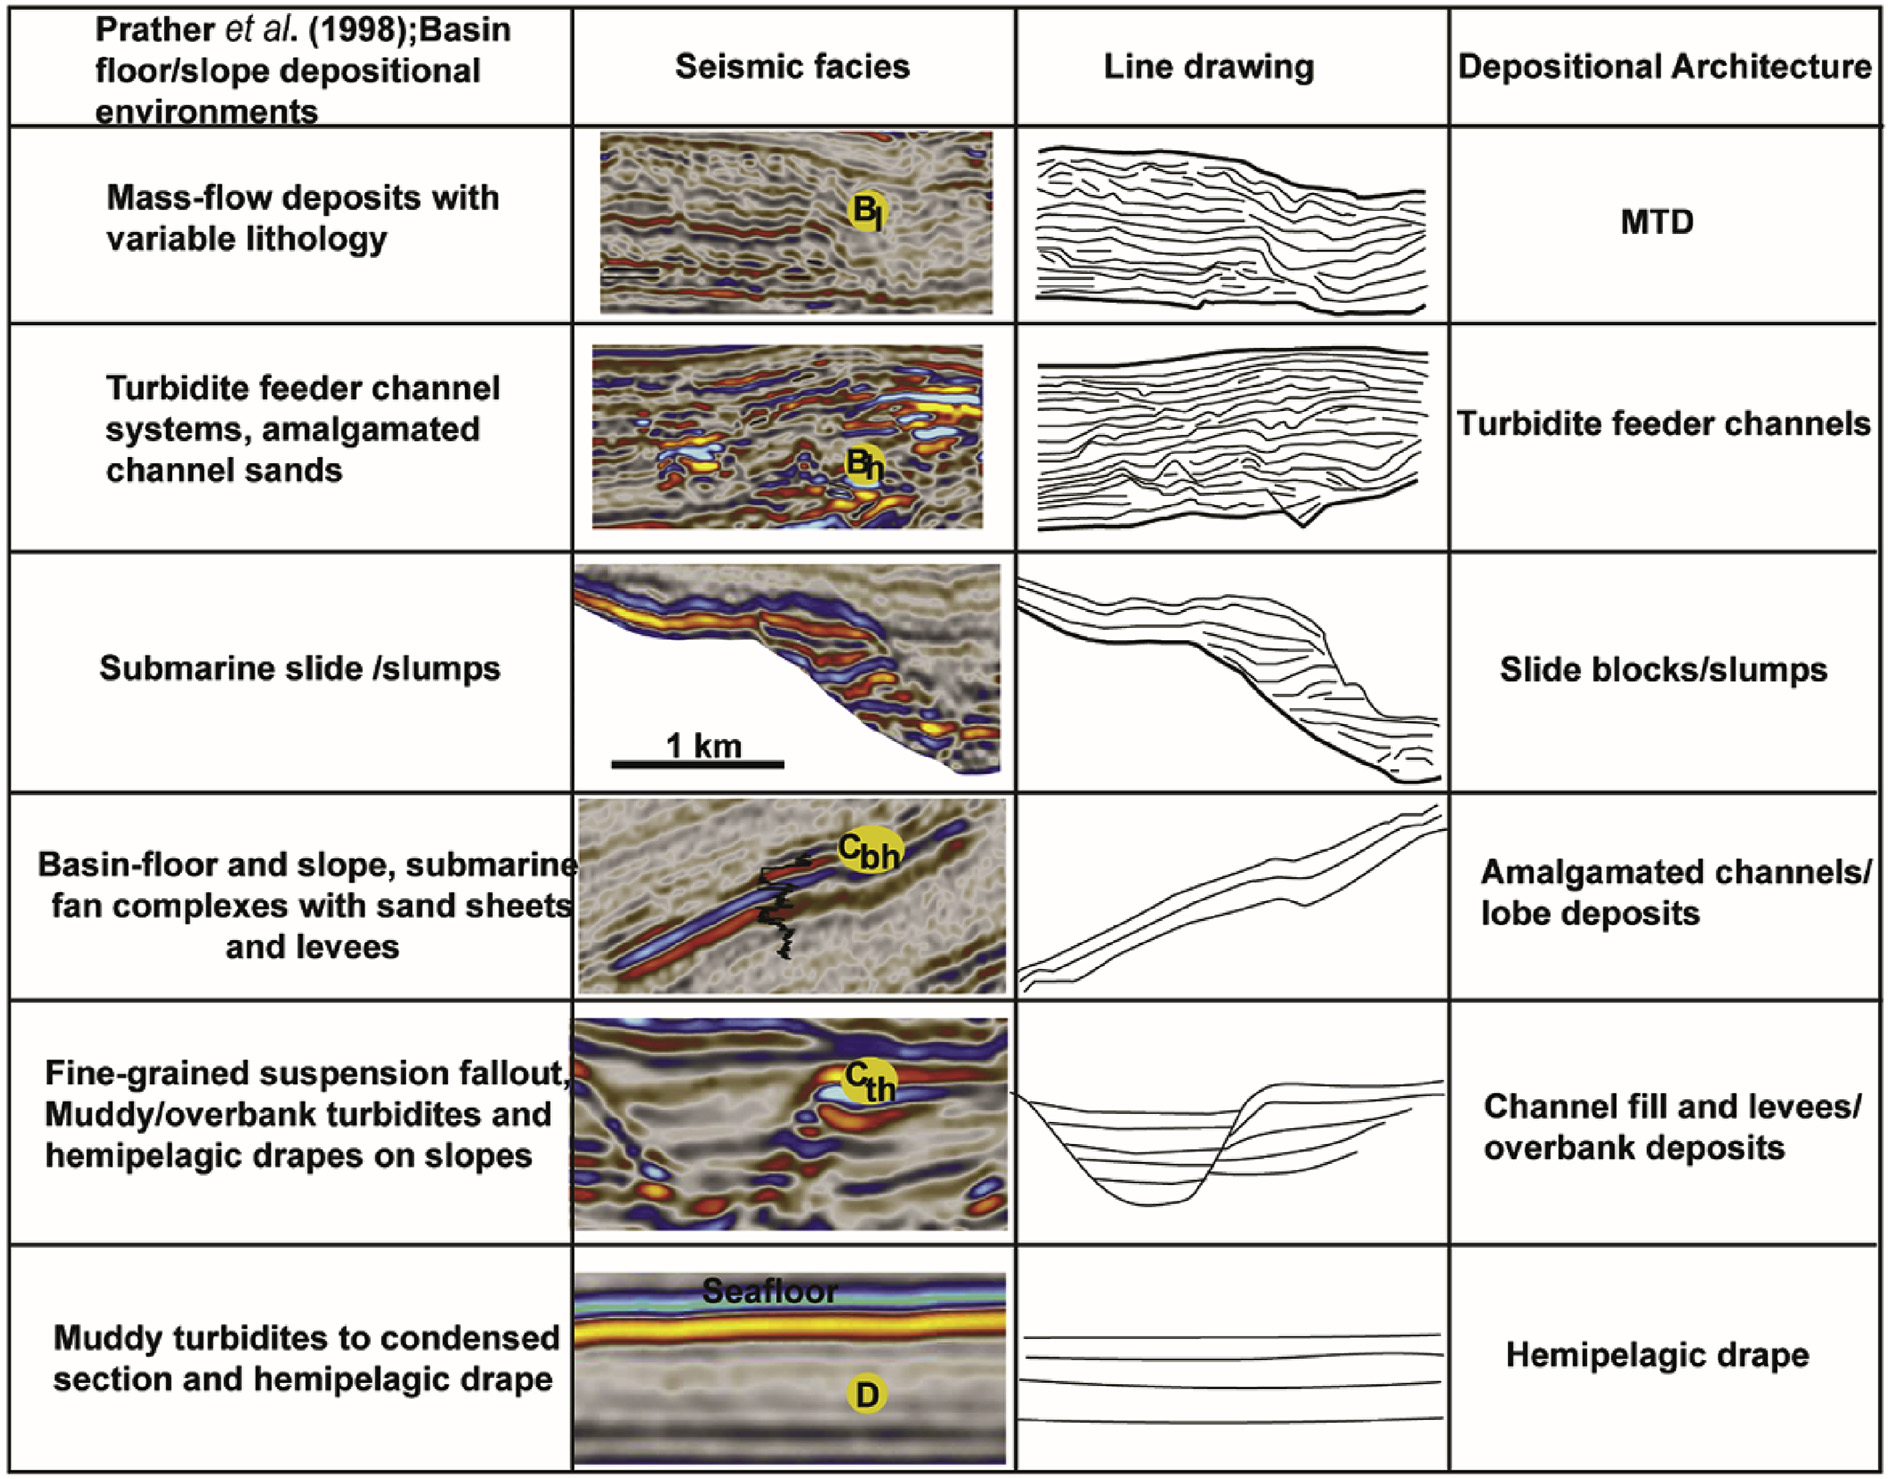
\includegraphics[width=0.75\linewidth]{Figures/0.3Seismic/Chima2019_Basin_trace_1.png}
    \caption[Offshore delta.]{Offshore delta. \textbf{Keywords: } High amplitude, medium amplitude, low amplitude, discontinuous, continuous, horizontal, dipping,  sub-parallel \citep{Chima2019}.}
    \label{fig:Chima2019-1}
\end{figure}

\begin{figure}[h!]
    \centering
    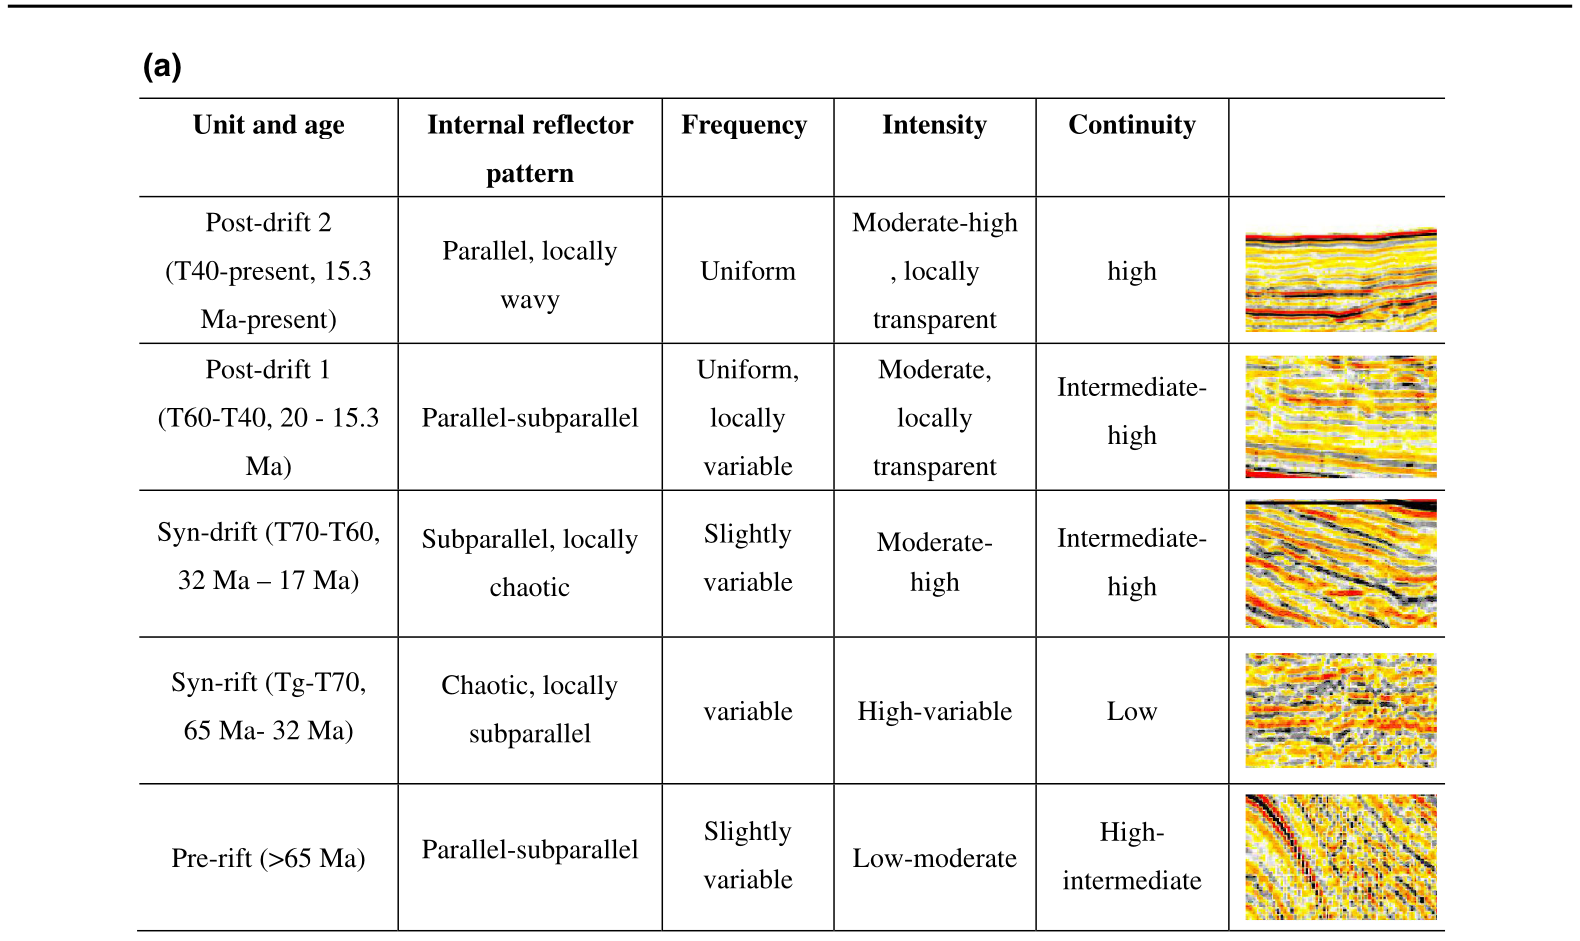
\includegraphics[width=0.9\linewidth]{Figures/0.3Seismic/Ding2014_Carbonates_trace_1.png}
    \caption[Tectono-sedimentary evolution (1).]{Tectono-sedimentary evolution (1). \textbf{Keywords: } Parallel, wavy, subparallel, chaotic, varied frequency, high continuity, low continuity, medium continuity, high amplitude, medium amplitude, low amplitude \citep{Ding2015}.}
    \label{fig:Ding2015-1}
\end{figure}

\begin{figure}[h!]
    \centering
    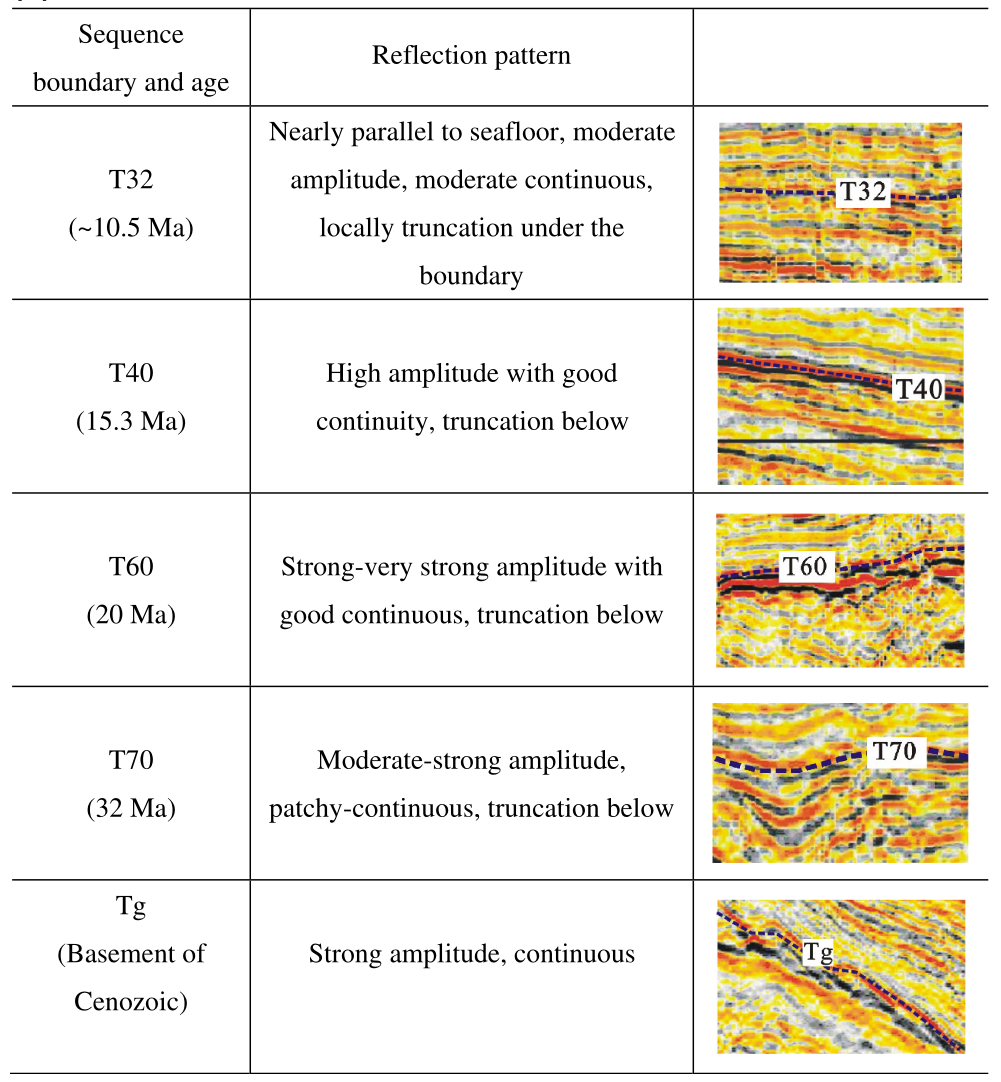
\includegraphics[width=0.9\linewidth]{Figures/0.3Seismic/Ding2014_Carbonates_trace_2.png}
    \caption[Tectono-sedimentary evolution (2).]{Tectono-sedimentary evolution (2). \textbf{Keywords: } Parallel, subparallel, high amplitude, medium amplitude, high continuity, medium continuity, truncation  \citep{Ding2015}.}
    \label{fig:Ding2015-2}
\end{figure}

\begin{figure}[h!]
    \centering
    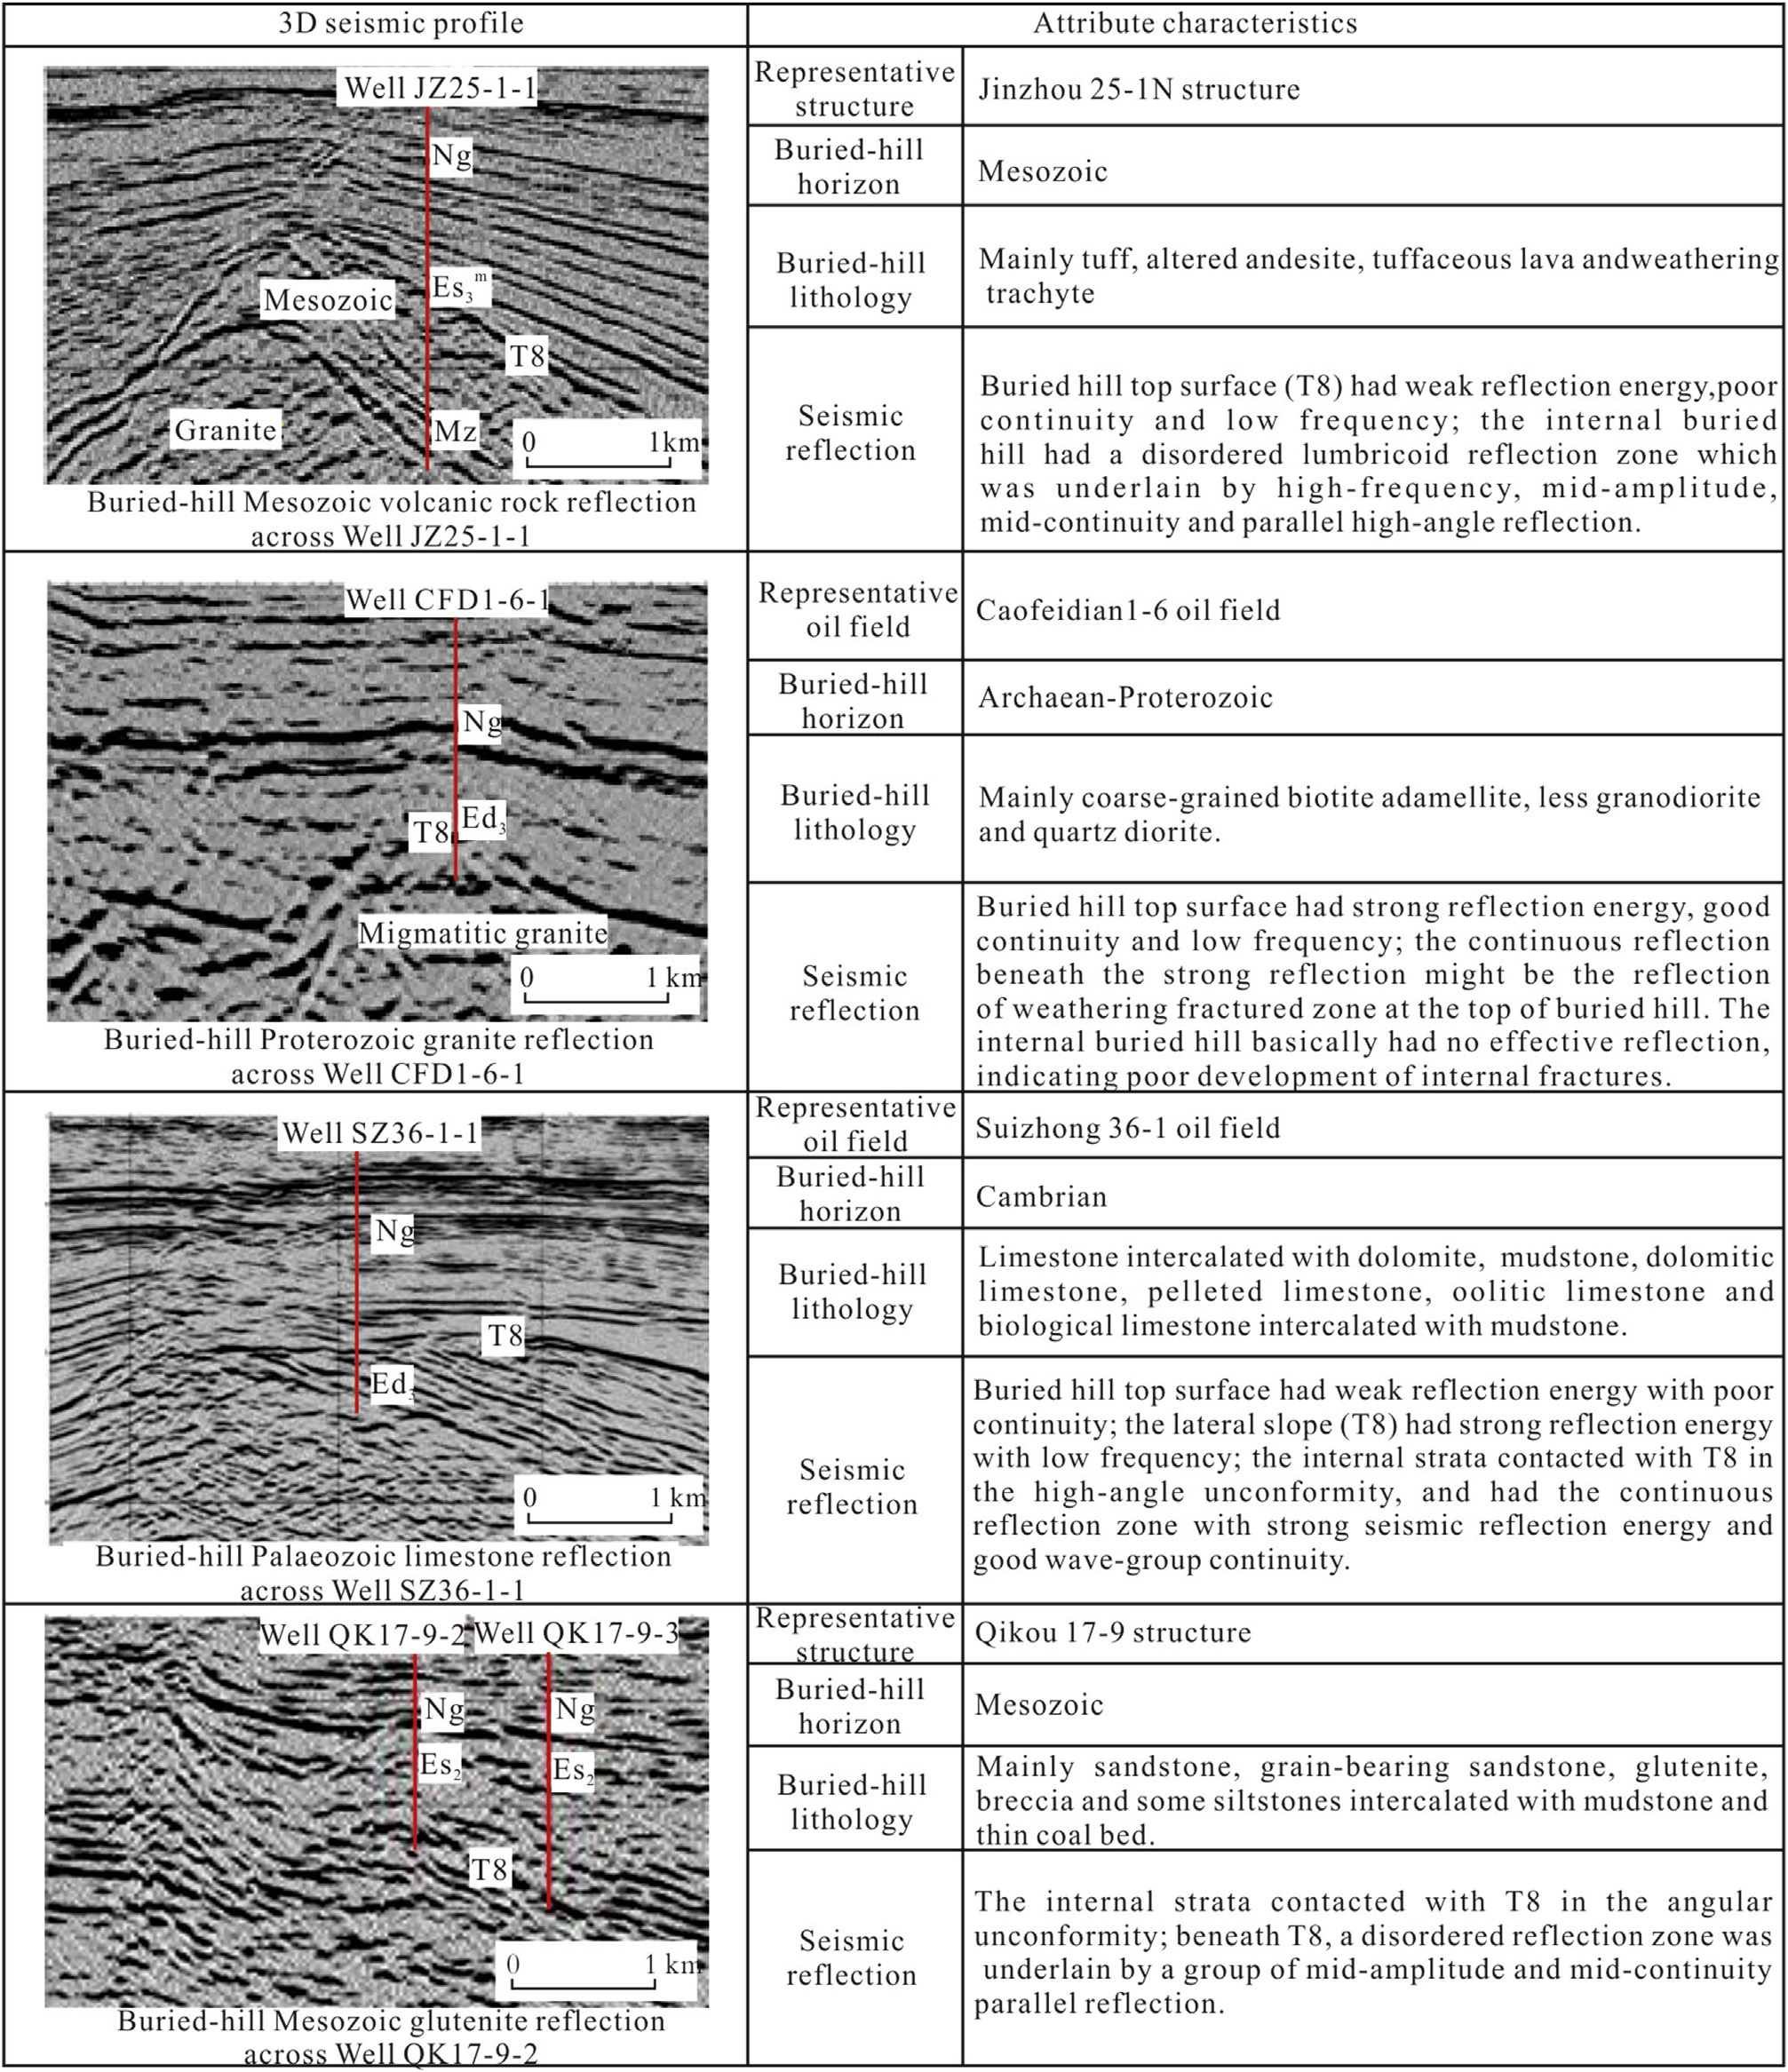
\includegraphics[width=0.9\linewidth]{Figures/0.3Seismic/Deng2017_buriedhill.png}
    \caption[Buried hill]{\textbf{Keywords: } Low amplitude, poor continuity, low frequency, medium amplitude, medium continuity, parallel, dipping, high amplitude, high continuity, chaotic, lateral slope, wavy \citep{Deng2017}.}
    \label{fig:Deng2017-1}
\end{figure}
\clearpage

\begin{figure}[h!]
    \centering
    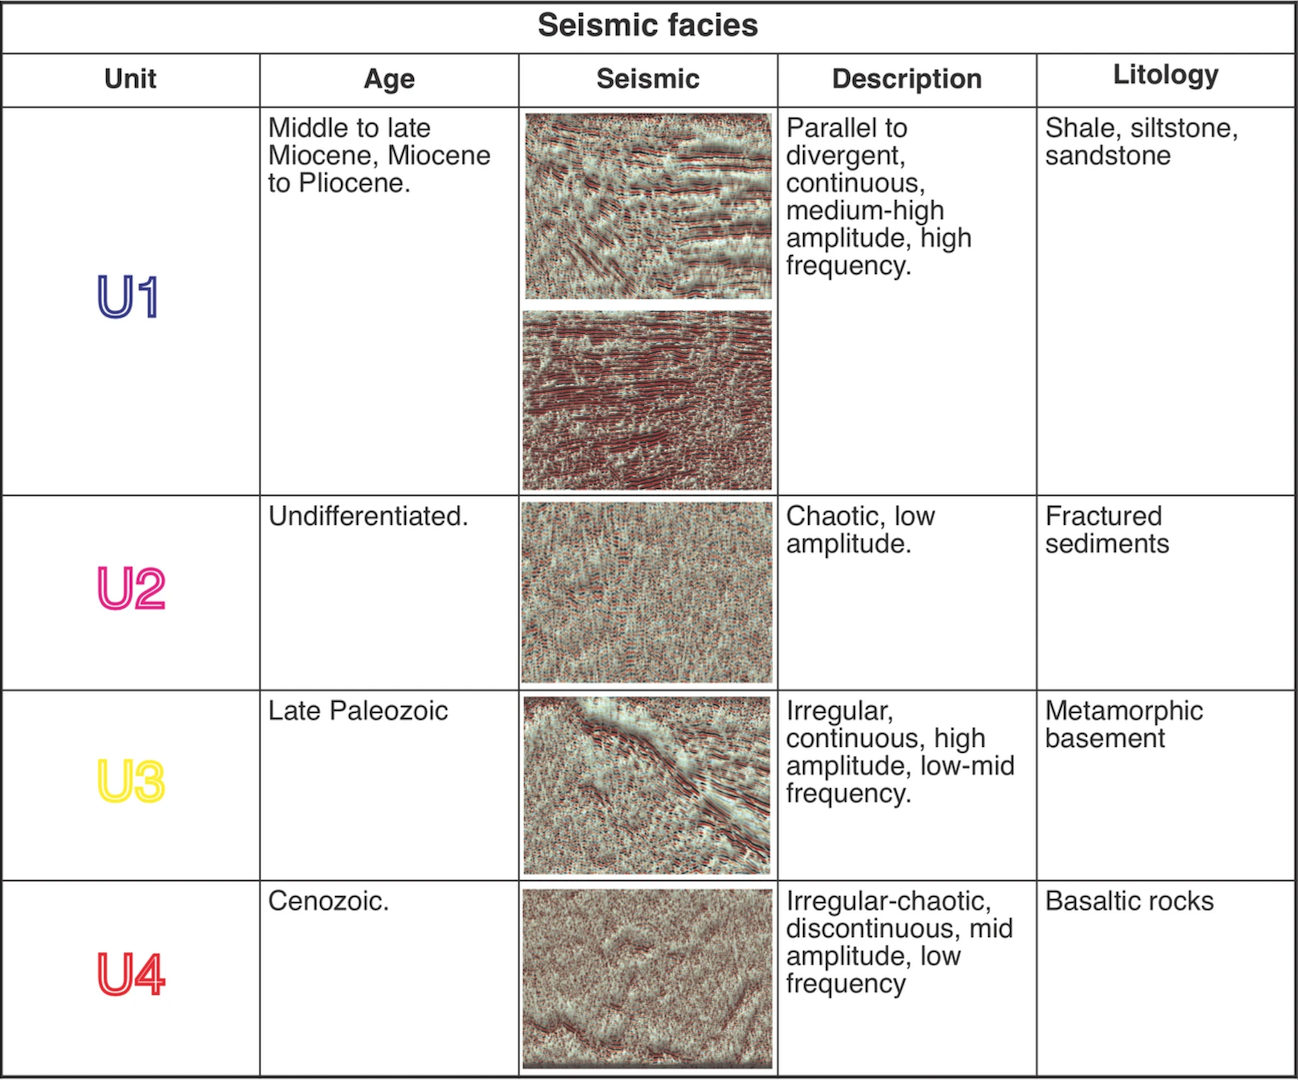
\includegraphics[width=0.9\linewidth]{Figures/0.3Seismic/Escobar2024_delta.png}
    \caption[Transform fault river delta.]{Transform fault river delta. \textbf{Keywords:} Parallel, divergent, continuous, medium amplitude, high amplitude, high frequency, chaotic, low amplitude, semi-continuous, low frequency, medium frequency \citep{Escobar2024}.}
    \label{fig:Escobar2024-1}
\end{figure}

%\begin{figure}[h!]
%    \centering
%    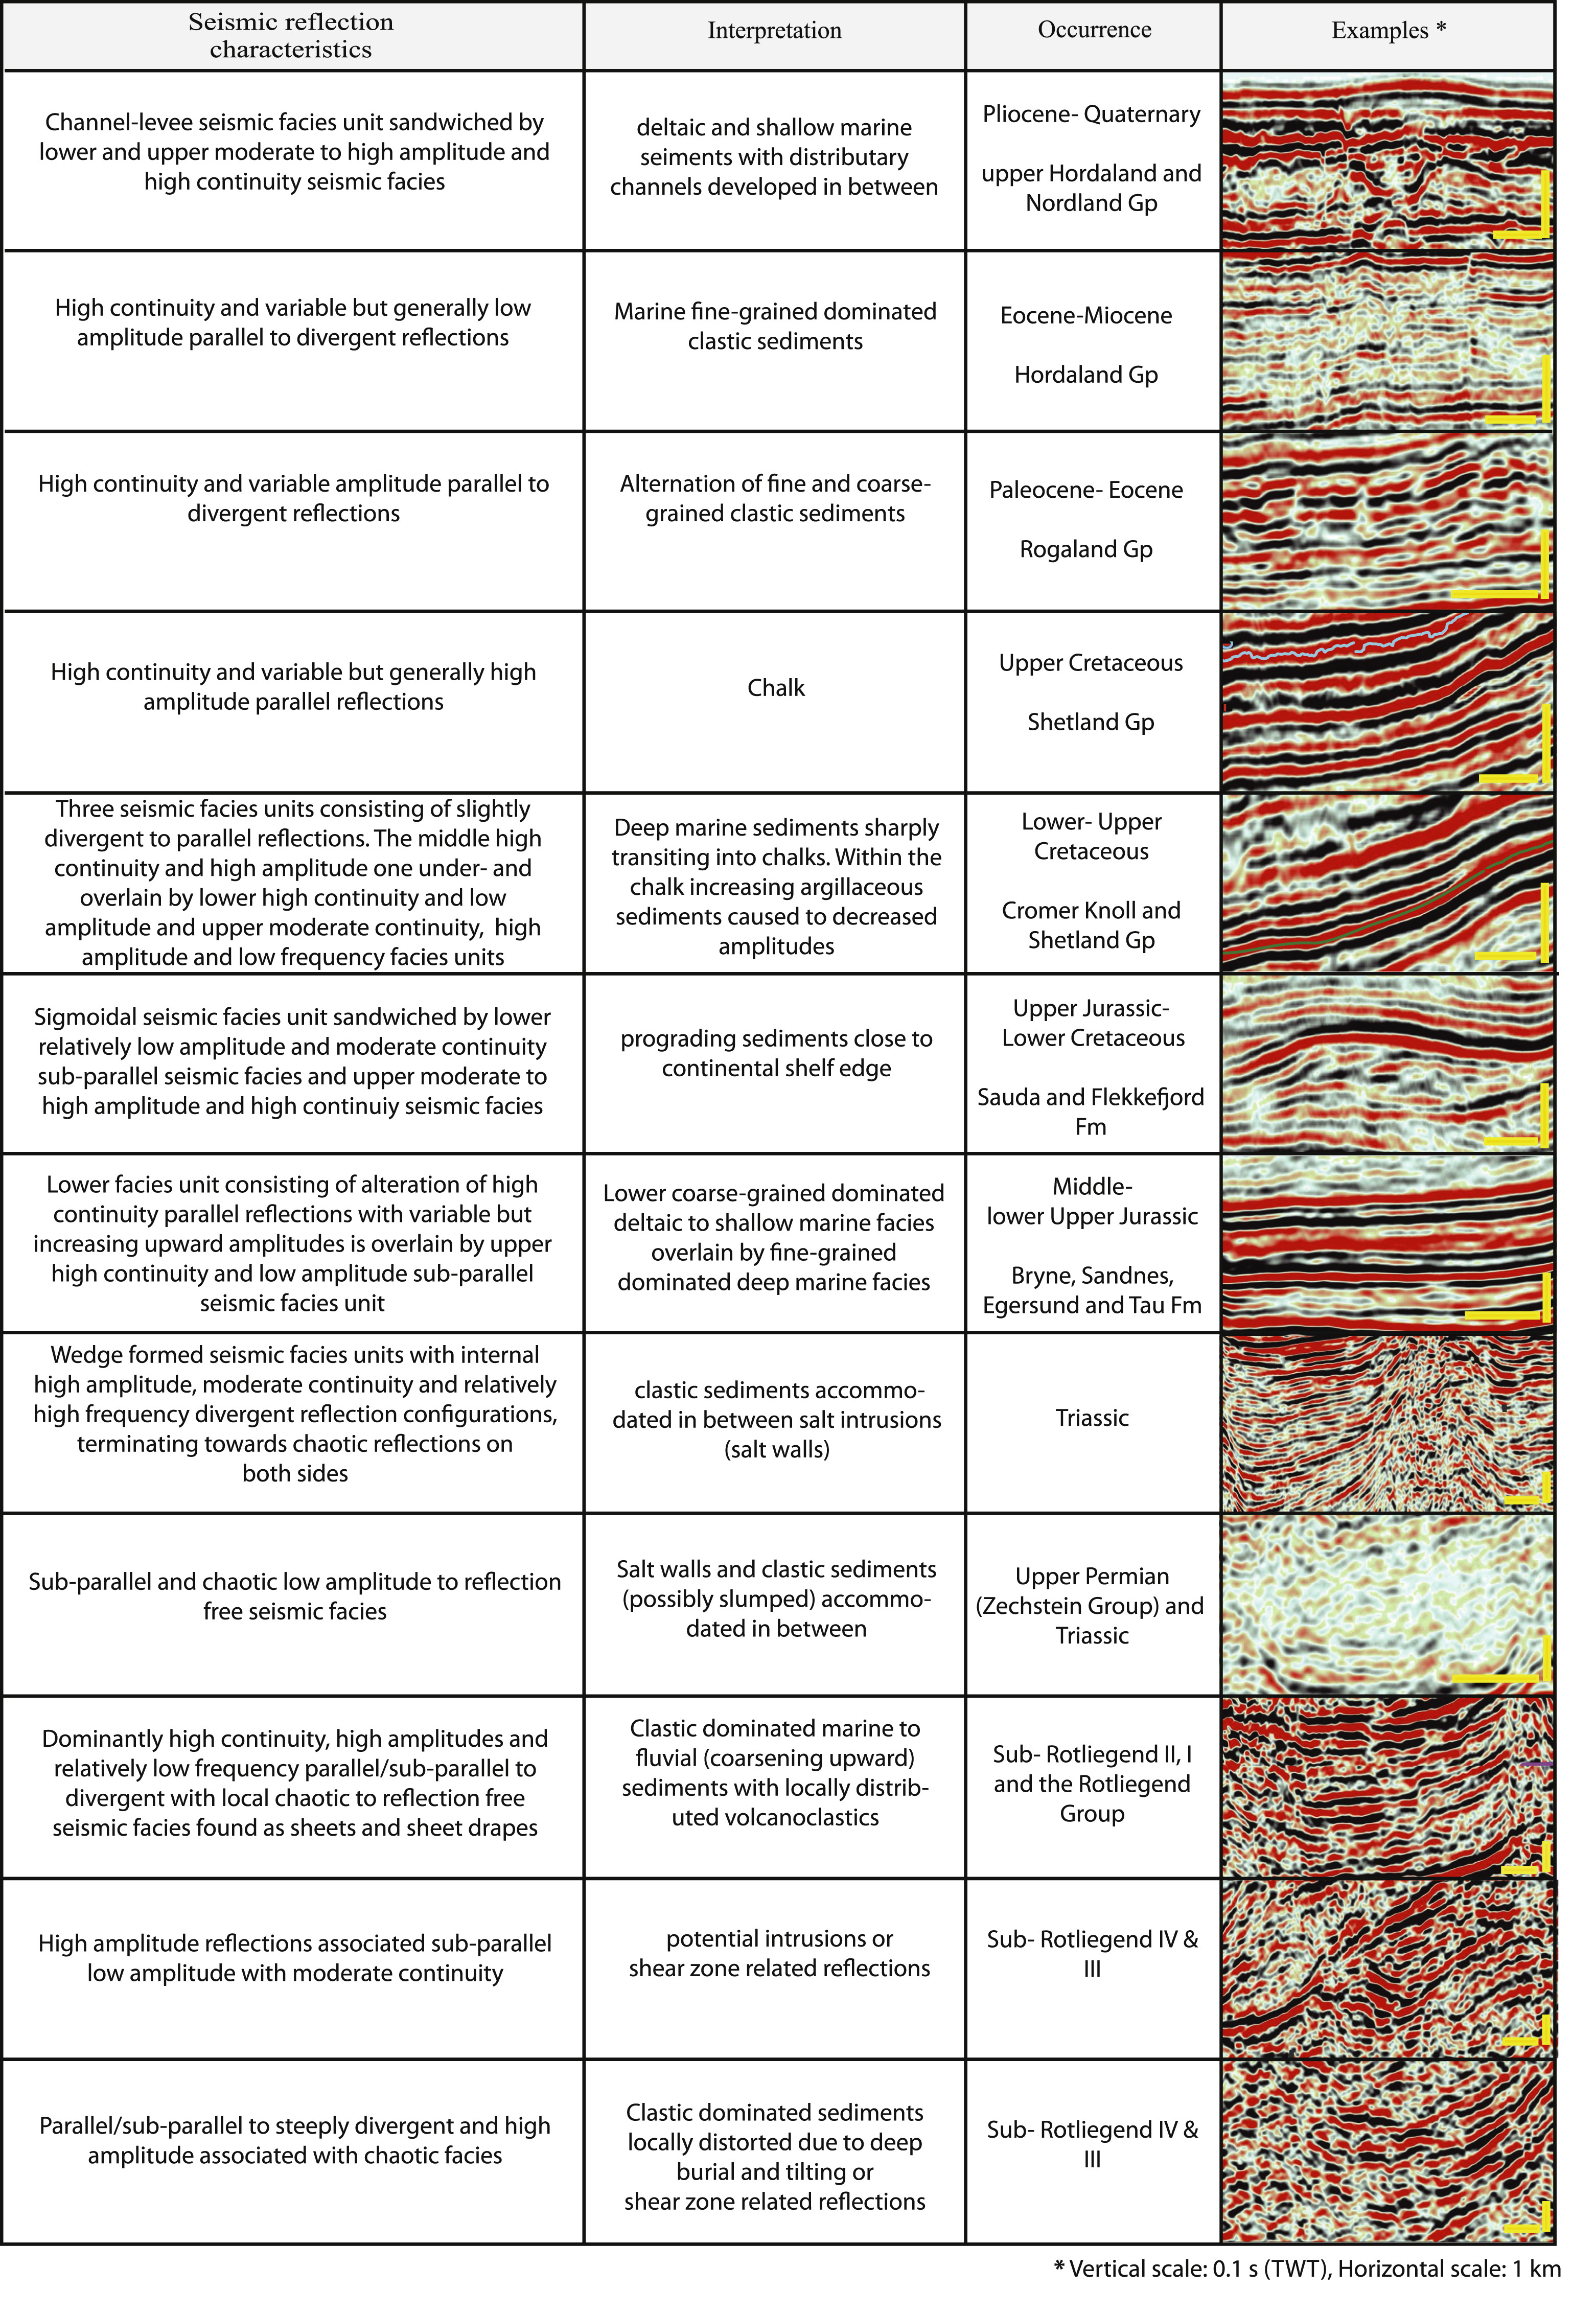
\includegraphics[width=0.75\linewidth]{Figures/0.3Seismic/kalani2020.jpg}
%    \caption[]{\textbf{Keywords: } \citep{Kalani2020}.}
%    \label{fig:Kalani2020}
%\end{figure}
%\clearpage
%\begin{figure}[h!]
%    \centering
%    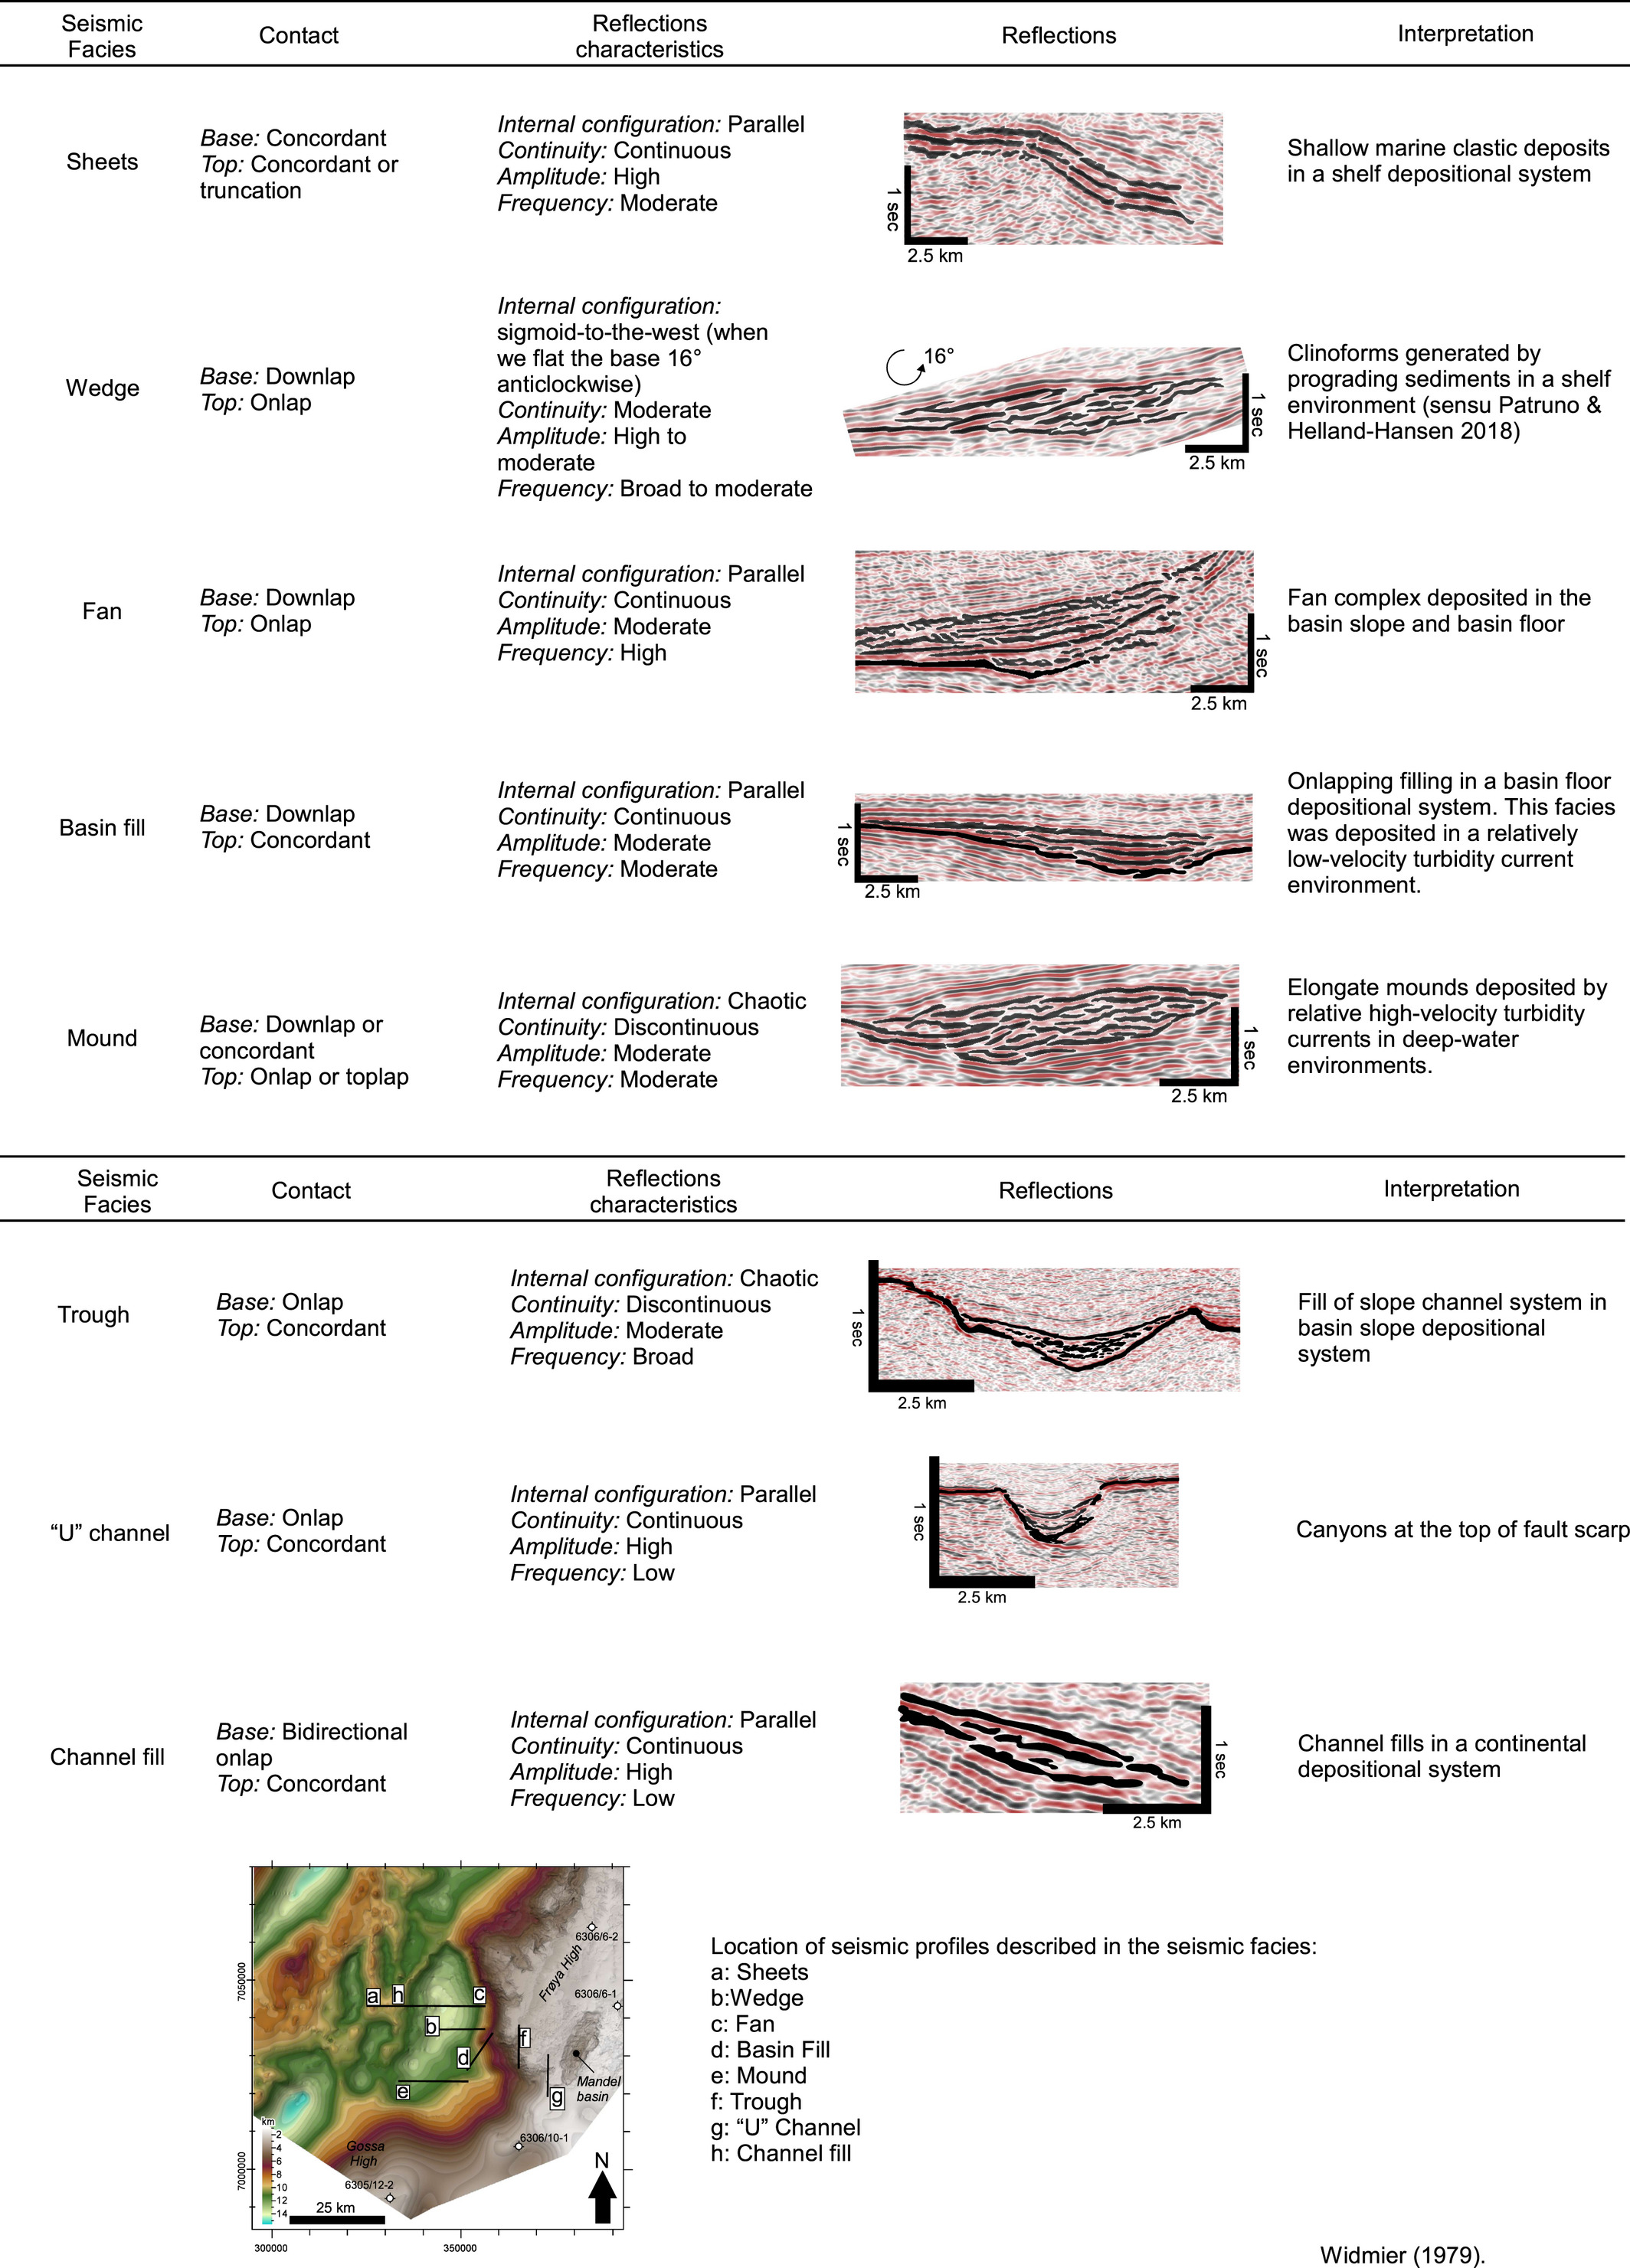
\includegraphics[width=0.75\linewidth]{Figures/0.3Seismic/Barrera2021.jpg}
%    \caption[]{\textbf{Keywords: } \citep{Barrera2021}.}
%    \label{fig:Barrera2021}
%\end{figure}